\def\mode{1}
\if0\mode
\documentclass[journal,twoside,web]{ieeecolor}
\usepackage{generic}
\else
\documentclass[journal,twoside]{IEEEtran}
\fi
\usepackage[english]{babel}
\frenchspacing

% *** MISCELLANEA PACKAGES ***
%
\usepackage{microtype}
\usepackage{setspace}
\usepackage{blindtext}
\usepackage{siunitx}
\pagestyle{headings}
\usepackage{titlecaps}
\Addlcwords{or with if of and an to -off off for in into the versus vs subject} % excluded words
\usepackage{comment}

% *** GRAPHICS RELATED PACKAGES ***
%
\usepackage[caption=false]{subfig}
\captionsetup[subfigure]{font={scriptsize,sf}}
\usepackage{graphicx}
\usepackage{fancyhdr} 
\usepackage{color}
\usepackage{epsfig}
\graphicspath{{Images/}}
\usepackage{tikz}
\usetikzlibrary{patterns,fit,matrix}
\usepackage{tikzscale}
\usepackage{scalerel}
\usetikzlibrary{arrows}
\usetikzlibrary{plotmarks}
\usetikzlibrary{svg.path}
\usetikzlibrary{shapes.multipart}
\usepackage{pgfplots}
\usepgfplotslibrary{fillbetween}
\pgfplotsset{compat=newest}
\pgfplotsset{every axis/.append style={
		label style={font=\Large},
		tick label style={font=\large}  
}}
\tikzstyle{int}=[draw, fill=black!10, minimum size=5em,thick]
\tikzstyle{init} = [pin edge={to-,thick,black}]

% *** ALIGNMENT PACKAGES ***
%
\usepackage{array}
\usepackage{stfloats}

% *** MATH PACKAGES ***
%
\let\proof\relax \let\endproof\relax
\usepackage{amsmath,amssymb,amsfonts,amsthm}
\numberwithin{equation}{section}
\usepackage{mathdots}
\usepackage{bbm,dsfont}
\usepackage{relsize}
\usepackage{nicefrac}
\usepackage{bbm}
\usepackage{mathtools}
\usepackage[mathscr]{eucal}

% *** SPECIALIZED LIST PACKAGES ***
%
\usepackage[ruled]{algorithm}
\usepackage{algpseudocode}
\usepackage{multirow}
\usepackage{makecell}
\makeatletter
\gdef\Shortstack{\@ifnextchar[\@Shortstack{\@Shortstack[c]}}
\gdef\@Shortstack[#1]#2{%
	\leavevmode
	\vbox\bgroup
	\baselineskip-\p@\lineskip 3\p@
	\let\mb@l\hss\let\mb@r\hss
	\expandafter\let\csname mb@#1\endcsname\relax
	\let\\\@stackcr\setlength{\baselineskip}{#2}%
	\@ishortstack}
\makeatother
\usepackage{booktabs}
\usepackage{tabularx}
\let\labelindent\relax
\usepackage{enumitem}

% *** FLOAT PACKAGES ***
%
\usepackage{float}
\usepackage[absolute]{textpos}

% *** PDF, URL AND HYPERLINK PACKAGES ***
%
\usepackage{url}
\usepackage{hyperref}
\makeatletter
\let\NAT@parse\undefined
\makeatother
\usepackage[capitalize]{cleveref}
\pdfminorversion=4

% *** CITATION PACKAGES ***
%
\usepackage{cite}

% link to ORCID
\newcommand\orcidicon[1]{\href{https://orcid.org/#1}{\includegraphics[scale=0.04]{orcid.pdf}}}

% correct bad hyphenation here
\hyphenation{op-tical net-works semi-conduc-tor}

% personalized commands
%!TEX root = ../book.tex
%%%%
%% section and chapter symbol
\newcommand{\secn}{\S}
\newcommand{\chp}{\S}

%%%% 
%% my environment for assumptions%%%
%%%%

\newenvironment{myassumptions}{%
   \begin{description}[style=multiline, leftmargin = 18pt, align=left]%
}{%
   \end{description}%
}
%%%%%
%%%%

%% ENUMERATED LABEL FOR ASSUMPTIONS
\makeatletter
\def\nl#1#2{\begingroup
    #2%
    \def\@currentlabel{#2}%
    \phantomsection\label{#1}\endgroup
}
\makeatother
%%%%%%
%%%%
%%

% to box multiple equations

\newenvironment{boxalign}[1]% 
{\ensuremath{
\begin{empheq}[box=\fbox]{align}
{#1}
\end{empheq}
}}


\newenvironment{advanced}{\small\fontfamily{ppl}\selectfont}{}
% ----- theorem-like environments                                                                                                   
\newtheorem{theorem}            {Theorem}[section]
\newtheorem{conjecture}            {Conjecture}[section]
\newtheorem{corollary}          [theorem]{Corollary}
\newtheorem{proposition}        [theorem]{Proposition}
\newtheorem{definition}         [theorem]{Definition}
\newtheorem{example}            [theorem]{Example}
\newtheorem{lemma}              [theorem]{Lemma}
\newtheorem{ass}                [theorem]{Assumption}
\newtheorem{remark}             [theorem]{Remark}
\newtheorem{result}             [theorem]{Result}



\newcommand{\normal}{\mathbfit{N}}  % this is the distribution
\newcommand{\uniform}{u}  % this is the rv

\newenvironment{boxresult}[1]% 
{
\begin{mdframed}
\par\noindent\textbf{#1:}\begin{rmfamily}\noindent}% 
{\end{rmfamily}
\end{mdframed}
} 

\newcommand{\pwe}{Complements and Sources}

%\newcommand{\Ep}{\E_\pdf}
\newcommand{\Ept}{\E_{\beliefm_\infty}}

\newcommand{\I}{\Pi}
\newcommand{\avg}{\phi}
\newcommand{\unavg}{L}
\newcommand{\dob}{\rho}  %dobrushin
\newcommand{\dist}{D}
\newcommand{\bias}{\operatorname{Bias}}
\newcommand{\var}{\operatorname{Var}}
\newcommand{\msd}{\operatorname{MSD}}

% prob, expectation

\newcommand{\rv}{x}
\newcommand{\rvY}{y}
\newcommand{\cdfb}{\bar{\cdf}}
\newcommand{\outcome}{\zeta}
\newcommand{\pdfX}{p}
\newcommand{\pdfY}{q}

\newcommand{\pdf}{p}
\newcommand{\cdf}{F}
\newcommand{\prob}{\mathbb{P}}
\newcommand{\E}                 {\Bbb{E}}
\newcommand{\bE}{\bar{\E}}
\renewcommand{\P}                 {\Bbb{P}}
\newcommand{\cov}{\operatorname{cov}}
\newcommand{\bre}{\mathbf{L}}
\newcommand{\pref}{q}  % reference prob method  density under \bar{P}

% state space
\newcommand{\grid}{\state}
\newcommand{\lowdim}{r}
\newcommand{\inp}{u}
\newcommand{\bstate}{\bar{\state}}
\newcommand{\onoisevar}{\sigma^2_\onoise}

\newcommand{\borelset}{S}
\newcommand{\tstate}{\tilde{\state}}

\newcommand{\obs}{y}
%\newcommand{\Obs}{\mathbf{y}}
\newcommand{\Obs}{\obs}

\newcommand{\snoise}{w}
\newcommand{\onoise}{v}
\newcommand{\statem}{A}
%\newcommand{\statem}{F}

\newcommand{\statemg}{\phi}
\newcommand{\obsmg}{\psi}
\newcommand{\snoisem}{\Gamma}

\newcommand{\obsm}{C}
%\newcommand{\obsm}{H}

%\newcommand{\obsmnew}{\psi}
\newcommand{\obsmnew}{H}
\newcommand{\level}{g}

%\newcommand{\onoisem}{D}
\newcommand{\onoisem}{D}
\newcommand{\inpm}{f}
\newcommand{\oinpm}{g}
\newcommand{\snoisecov}{Q}
\newcommand{\onoisecov}{R}
\newcommand{\onoisecovnew}{R}
\newcommand{\ar}{a} % AR coefficients
\newcommand{\arp}{s} % ar process

\newcommand{\state}{x}
\newcommand{\statespace}{\mathcal{X}}
\newcommand{\obspace}{\mathcal{Y}}
\newcommand{\statedim}{X}
\newcommand{\obsdim}{{Y}}

\newcommand{\mc}{r}  % markov chain of JMLS
\newcommand{\finals}{x} % reciprocal markov process

\newcommand{\fun}{\phi}
\newcommand{\funbar}{\psi}

\newcommand{\obsdummy}{y}

\newcommand{\identity}{I}



%% stoch convergence
\newcommand{\law}{\stackrel{\mathcal{L}}{=}}

% VARIATIONAL DISTANCE
\newcommand{\dvar}[2]{\|{#1}-{#2}\|_{\text{\tiny{TV}}}}
\newcommand{\dvarsq}[2]{\|{#1}-{#2}\|^2_{\text{\tiny{TV}}}}
\newcommand{\dvarn}{\| \cdot \|_{\text{\tiny{TV}}}}

% HMM parameters
\newcommand{\oprob}{B}
\newcommand{\tp}{P}
\newcommand{\utp}{\bar{\tp}}
\newcommand{\ltp}{\underline{\tp}}


\newcommand{\btp}{\bar{\tp}}
\newcommand{\jump}{J}
\newcommand{\duration}{D}
\newcommand{\sensm}{S^\model}

\newcommand{\eigenvec}{\nu}
%%

\newcommand{\finaltime}{N}
\newcommand{\btime}{\finaltime}


% models
\newcommand{\model}{\theta}
\newcommand{\modelpsi}{\psi}
\newcommand{\truemodel}{\model^o}
\newcommand{\modelem}{\model_\text{EM}}
\newcommand{\modelnr}{\model_\text{NR}}

\newcommand{\Model}{\Theta}
\newcommand{\lik}{L_\finaltime} % likelihood
\newcommand{\logl}{\mathcal{L}_\finaltime}  % log likeilhood
\newcommand{\aux}{\mathcal{Q}}  % EM algorithm Q aux likelihood

\newcommand{\beliefm}{\belief_\model}
\newcommand{\Mbelief}{\Pi_\infty}


\newcommand{\ubeliefm}{\ubelief^\model}
\newcommand{\likc}{\pdf(\obs_{1:\finaltime}| \model)}
\newcommand{\pdfm}{\pdf^\model}
\newcommand{\mle}{\model^*}
\newcommand{\ml}[1]{{#1}^*}
\newcommand{\oprobm}{\oprob^\model}
\newcommand{\tpm}{{\tp_\model}}
\newcommand{\nablam}{\nabla_\model}
\newcommand{\ardim}{M} % dimension of ar model
\newcommand{\sigmasnoise}{\sigma}

% radar
\newcommand{\range}{d}

% belief space
\newcommand{\belief}{\pi}
\newcommand{\beliefzero}{\belief}
\newcommand{\bbelief}{\bar{\pi}}
\newcommand{\ubelief}{{q}}
\newcommand{\upbelief}{\bar{\pi}}
\newcommand{\lbelief}{\underline{\pi}}

\newcommand{\lmean}{\underline{\state}}
\newcommand{\mean}{{\hat{\state}}}
\newcommand{\umean}{\bar{\state}}


\newcommand{\mat}{M}
\newcommand{\diff}{L^\epsilon}

%%%%%%%%%%

\newcommand{\Belief}{\Pi(\statedim)}
\newcommand{\back}{\beta}
\newcommand{\bay}[2]{\mathcal{B}[{#1},{#2}]}
\newcommand{\diagp}{P}


%social learning
\newcommand{\tbelief}{\pi^0}
\newcommand{\history}{\mathcal{H}}
\newcommand{\full}{\mathcal{F}}

\newcommand{\sigs}{\sigma}
\newcommand{\Bs}{R^\pi} 
\newcommand{\Bsl}{R^n}
\newcommand{\priv}{\eta}
\newcommand{\etaregion}{\kappa}

   \newcommand{\ca}{\cost_\action}
   \newcommand{\socialcost}{l}
   \newcommand{\ta}{\tilde{\action}}
   \newcommand{\sA}{\mathcal{A}}
   
   % incest 
   \newcommand{\quantized}{Q}
   
% Kalman filter variables
\newcommand{\kalmancov}{\Sigma}
\newcommand{\kalmangain}{K}
\newcommand{\lqgain}{L}
\newcommand{\kgain}{\bar{K}}  % this satisfies A L = kalmangain
\newcommand{\tr}{\normalfont{\text{trace}}}
\newcommand{\Sig}{S}   %  used for S_k in Kalman filter
\newcommand{\prederr}{\nu}
\newcommand{\ksgain}{G}

% delay variables
\newcommand{\delay}{\Delta}
\newcommand{\Delay}{\Delta}
\newcommand{\delaydim}{L}
\newcommand{\tpd}{\tp^{(\delay)}}
\newcommand{\dobs}{z}



\newcommand{\delaysetim}{\{1,2,\ldots,L-1\}}
\newcommand{\Delayset}{\{0 \text{ (announce change)} ,\D_1,\D_2,\ldots,\D_L\}}
\newcommand{\Delayseti}{\{0 \text{ (announce change)} ,1,2,\ldots, L\}}


% particle filter
\newcommand{\imp }{\pi}
\newcommand{\weight}{\omega}
\newcommand{\nw}{\tilde{\weight}}  % particle filter normalized weight
\newcommand{\ole}{\stackrel{\text{defn}}{=}}


% additive functional
\newcommand{\af}{S}  % ADDITIVE functional
\newcommand{\mf}{\mu}   % measure valued pdf of functional


\newcommand{\est}{\kappa}
\newcommand{\Est}{\boldsymbol{\kappa}}

\newcommand{\gtp}{\underset{\text{\tiny TP2}}{\geq}}
\newcommand{\gr}{\geq_r}
\newcommand{\lr}{\leq_r}
\newcommand{\gs}{\geq_s}
\newcommand{\ls}{\leq_s}






\newcommand{\filterd}{\sigma}
\newcommand{\filtern}{\alpha}
\newcommand{\filternum}{\gamma}
\newcommand{\filter}{T}
\newcommand{\bayes}{\mathcal{B}}

\renewcommand{\vec}{\operatorname{vec}}

\newcommand{\argmin}{\operatornamewithlimits{argmin}}
\newcommand{\argmax}{\operatornamewithlimits{argmax}}

\newcommand{\reals}{{\rm I\hspace{-.07cm}R}}
\newcommand{\R}{{\rm I\hspace{-.07cm}R}}
\newcommand{\N}{{\rm I\hspace{-.07cm}N}}
\newcommand{\continuous}{{\rm I\hspace{-.16cm}C}}

\newcommand{\F}{\mathcal{F}}   % sigma algebra

\newcommand{\beq}{\begin{equation}}
\newcommand{\eeq}{\end{equation}}
\newcommand{\nn}{\nonumber}

\renewcommand{\(}		{\left(}
\renewcommand{\)}		{\right)}


\newcommand{\Y}{\mathbf{Y}}

\renewcommand{\th}{\theta}
\newcommand{\Th}{\Theta}

\newcommand{\p}{\prime}

\newcommand{\one}{\mathbf{1}}
\newcommand{\ones}{\mathbf{1}}
\newcommand{\zero}{\mathbf{0}}


% tracking variables
\newcommand{\pos}{p}
\newcommand{\samt}{\Delta}
\newcommand{\jerk}{q}
\newcommand{\assoc}{a}

\newcommand{\f}{f} % false measurement

%%%%% continuous time


\newcommand{\bs}{\bar{\sigma}}
\newcommand{\osig}{\mathcal{Y}}
\renewcommand{\div} {{\operatorname{div}}}
\newcommand{\ftime}{T}
\newcommand{\gen}{Q}
\newcommand{\diag}{\textnormal{diag}}

\newcommand{\bop}{\mathcal L}
\newcommand{\fop}{\bop^*}

\newcommand{\pnoise}{\nu}
\newcommand{\rate}{\lambda}
\newcommand{\pois}{N}
\newcommand{\markpdf}{\pdf}
\newcommand{\marked}{z}
\newcommand{\event}{t}
\newcommand{\markspace}{\mathcal M}
\newcommand{\sigf}{\mathcal{F}}
\newcommand{\testf}{\phi}
\newcommand{\mart}{M}

\newcommand{\bq}{\bar{\ubelief}}
\newcommand{\be}{\bar{\epsilon}}
\newcommand{\bback}{\bar{\back}}

\newcommand{\forwardzakai}{q}
\def\la{\langle}
\def\ra{\rangle}


%structural filter
\newcommand{\gRm}{\succeq_M}
\newcommand{\lRm}{\preceq_M}
\newcommand{\uA}{\underline{A}}

\renewcommand{\i}{\mathbf{i}}
\renewcommand{\j}{\mathbf{j}}
\newcommand{\gtptwo}{\underset{\text{\tiny TP2}}{\geq}}
\newcommand{\ltptwo}{\underset{\text{\tiny TP2}}{\leq}}

\newcommand{\nm}{L}
\newcommand{\lR}{\preceq}
\newcommand{\gR}{\succeq}
\newcommand{\cons}{{\text{\bf Cons}}}
\newcommand{\consb}{\overline{\text{\bf Cons}}}
\newcommand{\conv}{{\text{conv}}}

\newcommand{\levels}{g}

\newcommand{\map}{\hat{\state}^{\text{MAP}}}
\newcommand{\lmap}{\underline{\state}^{\text{MAP}}}
\newcommand{\umap}{\bar{\state}^{\text{MAP}}}


% STOCHASTIC CONTROL
\newcommand{\Minimize}{\operatorname{Minimize}}
\newcommand{\marginal}{p}
\newcommand{\bmodel}{\bar{\model}}
\newcommand{\hQ}{\hat{Q}}

\newcommand{\ltwo}{\log_2}

%\newcommand {\brMet}{\ensuremath{\rho}} % the metric on the space \brSpc 
\newcommand{\sgain}{M}
\newcommand{\again}{N}
\newcommand{\fgain}{L}

\newcommand{\terminalcosta}{\cost_{\finaltime+1}}
\newcommand{\actions}{\action^\state}
\newcommand{\actionm}{\action^\obs}

\newcommand{\dpop}{L}
\newcommand{\cost}{c}
\newcommand{\covcost}{C}
\newcommand{\reward}{r}
\newcommand{\terminalcost}{\cost_\finaltime}
\newcommand{\Cost}{C}
\newcommand{\nlcost}{d}
\newcommand{\nlCost}{D}

\newcommand{\yi}{y^{(1)}}
\newcommand{\yii}{y^{(2)}}
\newcommand{\valueft}{\tilde{\valuef}}

\newcommand{\bmc}{\bar{m}}

\newcommand{\bQ}{\bar{Q}}
\newcommand{\bvalueb}{\bar{\valueb}}

\newcommand{\action}{u}
\newcommand{\baction}{\bar{\action}}
\newcommand{\actionspace}{\,\mathcal{U}}
\newcommand{\actiondim}{U}
\newcommand{\laspace}{\mathcal{A}}
%\newcommand{\cost}{c}
\newcommand{\totalcost}{J}
\newcommand{\exptotalcost}{J_{\bpolicy}}
\newcommand{\opttotalcost}{J_{\bpolicy^*}}
\newcommand{\discount}{\rho}

\newcommand{\region}{\mathcal{R}}
\def \con {{\beta}}
\def \rcon {{\gamma}}
\def \Con {{B}}
\def\param{{\alpha}}
\def \Z {{\cal Z}}
%%%% \def \a {{\alpha}}
\def \a {{\psi}}
\def\Param{{\boldsymbol{\alpha}}}
\def \Epi {{\E}_{\pi(\param)}}
 \def \G{{B}}
 \newcommand{\statpi}{\pi}
 \newcommand{\Ep}{\E_{\policy}}

\def\Policy{{\boldsymbol{\policy}}}
\newcommand{\policy}{\mu}
\newcommand{\optpolicyv}{\bpolicy^*}
\newcommand{\optpolicy}{\policy^*}
\newcommand{\bpolicy}{{\boldsymbol{\mu}}}
\newcommand{\optimaltotalcost}{J_{\optpolicy}}
\newcommand{\valuef}{V}
\newcommand{\valuefb}{\bar{\valuef}}
\newcommand{\valueb}{J}
\newcommand{\info}{\mathcal{I}}
\newcommand{\uV}{\underline{V}}

\newcommand{\bvalvec}{\bar{\gamma}}
\newcommand{\valvec}{\gamma}
\newcommand{\Valvec}{\Gamma}

\newcommand{\overlook}{\beta}
\newcommand{\blockprob}{q}
\newcommand{\augss}{\bar{\statespace}}
\newcommand{\terminal}{T}
\newcommand{\schRwd}{h}
\newcommand{\actionCost}{\cost}
\newcommand{\schHst}{\info}
\newcommand{\policySpc}{\mathcal{U}}
\newcommand{\schRwdFn}{J}

% stopping set
\newcommand{\stopset}{\mathcal{S}}

% POMDP (pom) quantities

\newcommand{\Jh}{J^{\text{h}}}
\newcommand{\Jo}{\bar{J}}
\newcommand{\thstate}{\state}
\newcommand{\thstatedim}{\statedim}

\newcommand{\pie}{\pi^{\epsilon_1,\epsilon_2,\ldots,\epsilon_{\statedim-1}}}
\newcommand{\pieone}{\pi^{\epsilon_1,\ldots\epsilon_j,\ldots, \epsilon_{\statedim-1}}}
\newcommand{\pietwo}{\pi^{\epsilon_1,\ldots\bar{\epsilon}_j,\ldots, \epsilon_{\statedim-1}}}


\newcommand{\Pimon}{\Pi_{\mathcal{M}}}
\newcommand{\beliefmon}{\belief_{\mathcal{M}}}

\newcommand{\ric}{\Gamma}
\newcommand{\iter}{n}
\newcommand{\iterfinal}{N}

\renewcommand{\time}{k}
\newcommand{\timet}{t}


\newcommand{\Hyperplane}{\mathcal{H}}


\newcommand{\Io}{{\Pi^o(X)}}
\newcommand{\Ib}{{\Pi^b(X)}}


\newcommand{\poly} {S}

\renewcommand{\l}{\mathcal{L}}


\newcommand{\unordered}{\sim}

\newcommand{\eye}{\textit{I}}
\newcommand{\bd}{\succeq_{\mathcal{B}}}
\newcommand{\aB}{R}
\newcommand{\tpone}{{\tp}}
\newcommand{\tptwo}{\bar{\tp}}

\newcommand{\tpe}{p}
\newcommand{\oprobe}{b}
\newcommand{\boprob}{\bar{\oprob}}

\newcommand{\noise}{n}
\newcommand{\asmp}{\textbf{A}}
\newcommand{\asmpg}{\bar{\text{A}}}

\newcommand{\statelvl} {h}
\newcommand{\sqg} {H}
\newcommand{\expcost} {C}

\newcommand{\cop}{C_o}
\newcommand{\thr}{\mathbf{\Gamma}}
\newcommand{\copomat}{\Gamma}

\newcommand{\uvalue}{\underline{V}}
\newcommand{\bvalue}{\overline{V}}
\newcommand{\valueaction}{Q}
\newcommand{\uvalueaction}{\underline{Q}}
\newcommand{\bvalueaction}{\overline{Q}}
\newcommand{\optvalue}{V}
\newcommand{\trid}{\Upsilon}
\newcommand{\filternorm}{\sigma}

\newcommand{\gc} {\succeq}
\newcommand{\lc} {\preceq}

%\newcommand{\ls}{_{s}{\le}}
\newcommand{\error}  {\eta}


\newcommand{\mus}{{\mu^*(\model)}}
\newcommand{\bmus}{{\mu^*(\bmodel)}}

\newcommand{\tcost}[1]{J_\mu^{(#1)}}


\newcommand{\rmm}{\rho_{\model,\bmodel}}

\newcommand{\lcost}{\underline{\textit{C}}}
\newcommand{\ucost}{\overline{\textit{C}}}
\newcommand {\uf} {\textit{f}}%{\underline{\textit{f}}\xspace}
\newcommand {\of} {\textit{g}}%{\overline{\textit{f}}\xspace}
\newcommand {\nooverlap} {\bar{\Belief}}
\newcommand {\setoverlap} {{\Pi_{O}}}
%\newcommand {\optpolicy} {\mu^*}
\newcommand {\policyu} {\overline{\mu}}
\newcommand {\policyl} {\underline{\mu}}


\newcommand{\yp}{y_{\pi;\model}^*}
\newcommand{\yps}{y_{\pi;\model,\bmodel}^*}
\newcommand{\ypsx}{y_{e_X;\model,\bmodel}^*}
\newcommand{\ytt}{y^*_{\model,\bmodel}}


\newcommand {\Timel} {\Gamma_l}
\newcommand {\Timev} {\Gamma_v}
%\newtheorem{mytheorem}{Theorem}
%\newcommand{\argmin}{\operatornamewithlimits{argmin}}
\newcommand{\basisvec} {\textit{e}}
\newcommand {\vect} {\textit{v}}
\newcommand {\percentloss} {\epsilon}
\newcommand {\approxpolicy} {\tilde{\mu}}
\newcommand{\bT}{\bar{T}}
\newcommand{\bsigma}{\bar{\sigma}}
\newcommand{\pomSt}{\ensuremath{s}}
\newcommand{\pomStSpc}{\ensuremath{S}}
\newcommand{\pomRwd}{\ensuremath{g}}
\newcommand{\pomTranMat}{\ensuremath{P}}
\newcommand{\pomObsMat}{\ensuremath{R}}
\newcommand{\pomAct}{\ensuremath{a}}
\newcommand{\pomActSpc}{\ensuremath{A}}
\newcommand{\pomObs}{\ensuremath{\theta}}
\newcommand{\pomObsSpc}{\ensuremath{\Theta}}
\newcommand{\pomHst}{\ensuremath{\Psi}}
\newcommand{\pomPol}{\ensuremath{\delta}}
\newcommand{\pomPolSpc}{\ensuremath{\Delta}}
\newcommand{\pomRwdFn}{\ensuremath{V}}
\newcommand{\pomHMM}{\ensuremath{\Phi}}
\newcommand{\pomPolVecSet}{\ensuremath{\Gamma}} % the PWLC representation of a policy
\newcommand{\pomPolVec}{\ensuremath{\gamma}}
\newcommand{\pomPolMapLB}{\ensuremath{\underline{\cal{H}}}} % lovejoy lower bound
\newcommand{\pomPolMapUB}{\ensuremath{\overline{\cal{H}}}} % lovejoy upper bound
\newcommand{\pomPolMap}{\ensuremath{\mathcal{H}}}

\newcommand{\comAct}{\pomAct} %
\newcommand{\comActSpc}{\pomActSpc}
\newcommand{\comObs}{\pomObs}
\newcommand{\comObsSpc}{\pomObsSpc}
\newcommand{\comPol}{\pomPol}
\newcommand{\comPolSpc}{\pomPolSpc}
\newcommand{\comRwdFn}{\pomRwdFn}
\newcommand{\obsMat}{R}



\newcommand{\gl}{\geq_{L_i}}
\newcommand{\glp}{\geq_{L_{i+1}}}

\newcommand{\glx}{\geq_{L_x}}
\newcommand{\glX}{\geq_{L_X}}
\newcommand{\glone}{\geq_{L_1}}


\newcommand{\bp}{{\bar{\pi}}}
%%
%grad
\def \La {{\cal L}}
\def \GF{{\widehat{\nabla C}^{\text{WD}}}}
\def \GS{{\widehat{\nabla C}^{\text{Score}}}}


%% SPSA
\newcommand{\wderiv}{g}
%\newcommand{\deriv}{L}
\newcommand{\hphi}{\hat{\phi}}
\newcommand{\nablat}{\widehat{\nabla}_{\phi}}
\newcommand{\direction}{\omega}

%%%%
%Sensor scheduling
\newcommand{\ac}{\tt{active}}
\newcommand{\co}{\tt passive}
\newcommand{\pr}{\tt predict}
\newcommand{\fa}{\rho^{\text{\ac}}}
\newcommand{\fc}{\rho^{\text{\co}}}
\newcommand{\fp}{\rho^{\text{\pr}}}
\newcommand{\ha}{r^{\text{\ac}}}
\newcommand{\hc}{r^{\text{\co}}}
\newcommand{\hp}{r^{\text{\pr}}}
\newcommand{\use}{n}
\newcommand{\tar}{z}

%%% quickest detection
%%%%%%
\newcommand{\epoch}{\tau}
\newcommand{\D}{D}
\newcommand{\delayset}{\{\D_1,\D_2,\ldots,\D_L\}}
\newcommand{\delayseti}{\{1,2,\ldots,L\}}
\newcommand{\kstar}{k^*}
\newcommand{\changetime}{\tau^0}
\newcommand{\falsealarm}{{f}}
\newcommand{\Vb}{\bar{V}}
\newcommand{\Pp}{\P_\mu}
\newcommand{\Cb}{\bar{C}}
\newcommand{\risk}{\epsilon}
%%%%
\newcommand{\stepsize}{\epsilon}

\newcommand{\A}{\mathbb{A}}
%%%%

%%%radar
\newcommand{\bkalmancov}{\bar{\Sigma}}
\newcommand{\price}{\nu} %{\mathbf{\nu}}
\newcommand{\Mu}{\boldsymbol{\mu}}
\newcommand{\grnew}{\succeq}
\newcommand{\gsnew}{\succ}
\newcommand{\lrnew}{\preceq}
\newcommand{\Q}{\mathcal{Q}}
\newcommand{\bt}{\underline{\theta}}
\newcommand{\lstar}{{l^*}}
\def\Lyapunov{{\cal L}}
\def\Ricatti{{\cal R}}
\def\pdfmat{\mathcal{M}}
%%%
%bandit
\newcommand{\numtarget}{L}
\newcommand{\target}{l}
\newcommand{\delt}{\delta}

%%%%%%%%

%%% disc opt %%
\newcommand{\bm}{w}
\newcommand{\globalopt}{\mathcal{G}}
\newcommand{\cd}{(\cdot)}
%\newcommand{\br}{\boldsymbol{b}^{\gamma}}
\newcommand{\br}{{b}^{\gamma}}
\newcommand{\bbr}{b^{\gamma}}
\newcommand{\boldf}{f}
\def\z{\mathbf{z}}
\def\lb{\left[}
\def\rb{\right]}
\def\lbr{\left\lbrace}
\def\rbr{\right\rbrace}
\def\RR{{\mathbb{R}}}
\newcommand{\pp}{{\mathbb P}}
\newcommand{\maxdiff}{D}

\newcommand{\score}{S}
\newcommand{\batchsize}{N}
\newcommand{\infodelta}{\info^\Delta}

%\newcommand{\degreelink}{\alpha}
\newcommand{\degreelink}{\th}
%%%%

%%%
%% primal dual
%%

\newcommand{\penaltyweight}{\Delta}

%%%%%
%%
%%% part 4  commands  %%%
%%%%
\def\ph{\varphi}
\newcommand{\M}{{\cal M}}
\newcommand{\lbar}{\overline}
\newcommand{\wdt}{\widetilde}

%\def\l{\Big|}

%\def\r{\Big|}
\newcommand{\ad}{&\!\!\!\disp}
\newcommand{\aad}{&\disp}
\newcommand{\barray}{\begin{array}{ll}}
\newcommand{\earray}{\end{array}}
\newcommand{\disp}{\displaystyle}

\newcommand{\h}{{\ell}}
\def\cd{(\cdot)}
\newcommand{\e}{\varepsilon}
\newcommand{\tth}{\tilde{\th}}
%%%
%%%
%% population dynamics and social network
\newcommand{\numagents}{M}

\newcommand{\nature}{\state}
\newcommand{\pop}{\theta}
\newcommand{\bpop}{\bar{\pop}}
\newcommand{\mpop}{\bar{\pop}}
\newcommand{\popspace}{\Theta}
\newcommand{\pa}{\alpha}

\newcommand{\network}{G}
\newcommand{\Vertexset}{V}
\newcommand{\vertexnum}{\numagents}
\newcommand{\vertexset}{\{1,2,\ldots,\vertexnum\}}
\newcommand{\edgeset}{E}
\newcommand{\degdist}{\rho}
\newcommand{\nodem}{m}
\newcommand{\degreediff}[1]{D^{(#1)}}
\newcommand{\atp}{\bar{\tp}}
\newcommand{\ed}{\bar{A}}

\newcommand{\wdh}{\widehat}


%%%% social learning chapter
 
\newcommand{\Req}{\mathcal{R}}
\newcommand{\poll}{\Req_{L}}
\newcommand{\additional}{\mathcal{E}}
\newcommand{\cbelief}{l^0}
\newcommand{\logoprob}{o}
\newcommand{\obseq}{\mathcal{Y}}
\newcommand{\omat}{\mathcal{O}}
\newcommand{\loprob}{\bar{R}}


%% afriat
   \newcommand{\probe}{\belief}
\newcommand{\response}{a}
\newcommand{\responseb}{\bar{x}}
\newcommand{\utility}{V}
\newcommand{\budget}{I}
\newcommand{\dataset}{\mathcal{D}}
    \newcommand{\norm}[1]{\lVert#1\rVert}
\newcommand{\tindx}{k}
\newcommand{\Tindxter}{\finaltime}


%%% mean field

\newcommand{\mtg}{\nu}
%\newcommand{\dev}{\Delta}
\newcommand{\dev}{\tilde{\theta}}


%%% search
\newcommand{\blocked}{b}

%% multivariate POMDP


\newcommand{\Sc}{\statespace}


\newcommand{\eprob}{\gamma}
\newcommand{\suffstat}{\eta}
\newcommand{\simplex}{\Pi}

\newcommand{\batch}{\iota}
\newcommand{\bsize}{N}
\newcommand{\bindex}{n}

\newcommand{\weightnl}{\alpha}

\newcommand{\Vt}{V(\filter(\pi,p,a))}

\newcommand{\sigfilter}{\filterd(\pi,p,a)}

\newcommand{\moncost}{c_o}
\newcommand{\monprice}{p}
\newcommand{\monreward}{c_\monprice}
\newcommand{\rewardv}[1]{c_{\monprice,#1}}
\newcommand{\rewv}{r_\monprice}


\newcommand{\riskf}{\mathbf{R}}
%\newcommand{\riskt}{\tilde{\E}}
\newcommand{\riskt}{\mathcal{R}}

\newcommand{\bfun}{\bar{\fun}}
%\newcommand{\det}{\operatorname{det}}


\title{{\titlecap{can decentralized control outperform centralized?} \\ \titlecap{the role of communication latency}}}

\author{Luca~Ballotta\textsuperscript{\orcidicon{0000-0002-6521-7142}}, %~\IEEEmembership{Graduate~Student~Member,~IEEE},\\%
	Mihailo~R.~Jovanovi\'c\textsuperscript{\orcidicon{0000-0002-4181-2924}},~\IEEEmembership{Fellow,~IEEE}, and %
	Luca~Schenato\textsuperscript{\orcidicon{0000-0003-2544-2553}},~\IEEEmembership{Fellow,~IEEE}%
	\thanks{
		This work has been partially supported
		by the Italian Ministry of Education, University and Research (MIUR) through
		the PRIN project no. 2017NS9FEY entitled ``Realtime Control of 5G Wireless Networks'', and through
		the initiative "Departments of Excellence" (Law 232/2016), and by
		the US National Science Foundation (NSF) under Awards ECCS-1708906 and ECCS-1809833.
		Views and opinions expressed in this work are of the authors and may not reflect those of the funding institutions.}%
	\thanks{Luca Ballotta and Luca Schenato are with the Department of Information Engineering, University of Padova, 35131 Padova, Italy
		(e-mail: ballotta@dei.unipd.it; schenato@dei.unipd.it)}%
	\thanks{Mihailo R.\ Jovanovi\'c is with the Ming Hsieh Department of Electrical and Computer Engineering,
		University of Southern California, Los Angeles, CA 90089 USA (e-mail: mihailo@usc.edu)}
}

\if0\mode
\markboth{IEEE Transactions on Control of Network Systems, VOL. XX, NO. XX, XXXX XXXX}
{Ballotta \MakeLowercase{\textit{et al.}}: can decentralized control outperform centralized? the role of communication latency}
\fi

\begin{document}
	
	\if1\mode
	\begin{textblock}{20}(-2,0.05)
		\footnotesize
		\centering
		\setstretch{1}
		This article has been accepted for publication on the IEEE Transactions on Control of Network Systems.\\
		Please cite the paper as: L. Ballotta, M. R. Jovanovi\'c, and L. Schenato,\\
		“{\titlecap{can decentralized control outperform centralized?} \titlecap{the role of communication latency}}”,\\
		IEEE Transactions on Control of Network Systems, 2023.\\
		%		Link to article abstract: \url{}
	\end{textblock}
	\fi
	
	\if0\mode
	\bstctlcite{MyBSTcontrol}
	\fi
	
	\maketitle
	\begin{abstract}
\label{sec:abstract}

%% 1. what is the problem 
Scientific applications that run on leadership computing facilities often face the challenge 
of being unable to fit leading science cases onto accelerator devices due to memory constraints 
(memory-bound applications).
%
% 2. what is your solution 
In this work, the authors studied one such US Department of Energy mission-critical condensed matter 
physics application, Dynamical Cluster Approximation (DCA++), and this paper discusses how device memory-bound challenges were successfully reduced  by proposing an effective 
``all-to-all'' communication method---a ring communication algorithm. 
%
This implementation takes advantage of acceleration on GPUs and remote direct memory access (RDMA) for fast data exchange between GPUs. 
%
\\Additionally, the ring algorithm was optimized with sub-ring communicators
and multi-threaded support to further reduce communication overhead and 
expose more concurrency, respectively.
%
% 3. What's the cherry-picked evaluation result you want to mention
The computation and communication were also analyzed 
by using the Autonomic Performance Environment for Exascale 
(APEX) profiling tool,  and this paper further discusses the 
performance trade-off for the ring algorithm implementation. 
%
The memory analysis on the ring algorithm shows that the allocation size for the authors' most 
memory-intensive data structure per GPU is now reduced to $1/p$ of the original size, where $p$ is the number of GPUs in the ring communicator.
%
The communication analysis suggests that 
the distributed Quantum Monte Carlo execution time grows linearly as sub-ring size increases, and the cost of messages passing through the network interface connector could be a limiting factor.


%
% \todoRed{Ronnie: Next sentence needs rewrite, too much information about Green's function that no one knows in the abstract; recommend generalizing.} \emph {However, DCA++ is currently facing memory-bound challenge as 
% a larger device array $G_t$ is limited by device memory size, where
% $G_t$ is a two-particle Green's function that allows condensed matter
% scientists to explore larger and more complex (higher fidelity)
% physics cases.}

\end{abstract}

\keywords{DCA++, Quantum Monte Carlo, GPU Remote Direct Memory Access, memory-bound issue, exascale machines}

	\section{Motivations for Empirical Study}
\label{sec:motivations}
The key question that we try to answer is when and why we should use standard
iteration space tiling over cache oblivious tiling.  The two approaches
perform similar partitioning of the iteration space, but the schedules given
to the partitions are different.  Theoretically, cache oblivious code seems to
have advantages over iteration space tiling.  However, many factors complicate
the actual performance, which made our initial experiments difficult to
interpret.  In this section, we describe the obstacles between the theory and
practice we have identified.

We use Single-Level Tiling (SLT) for iteration space tiling, and Cache
Oblivious Tiling (COT) for cache oblivious techniques in this
paper, which are further described in Section~\ref{sec:background}.

\paragraph{Recursion Overhead} This is a well-known overhead of
COT~\cite{yotov2007experimental}.  The recursion introduces overheads, such as
function call overhead, and increased register pressure.  Furthemore, the
functions force inter-procedural analysis/optimization, known to be more
difficult for compilers well.  Thus, the leaf tiles must be ``sufficiently
large'' to avoid excessive overhead due to the recursion.

 \paragraph{Recursive Split Constraints the Tile Sizes} In typical cache
 oblivious algorithms, the problem is recursively split into halves in each
 dimension. This is in fact a rather coarse-grained exploration of the
 hierarchical partitioning of the iteration space. For instance, if the
 current problem size is $B^3$, then the next sub-problem would be
 $(\frac{B}{2})^3$.  If the best problem size for utilizing a level of cache
 is $(B-x)^3$ where $x\ll \frac{B}{2}$ then the subproblems due to
 divide-and-conquer will not match the best.  This is another factor that
 necessitates fine tuning of leaf tile sizes even for COT, since the utilization
 rate of L1 cache has strong impact on performance.  

%\paragraph{COT Leads to Imbalanced Tiles} Current COT tools recursively split
%the problem into halves in each dimension.  If the original bounds are not
%powers of two, every power-of-two leaf will be paired with a non-power-of-two
%leaf.  Since leaf tile sizes are often carefully tuned, thismeans that half
%the leaves will be suboptimal.  Our code generator incorporates a simple
%optimization that ensures that such suboptimal leaf nodes only occur at the
%boundaries of the iteration space.

\paragraph{COT has more Conflict Misses} The divide-and-conquer execution
order may negatively affect cache interference, especially with high
dimensional data.  This happens when the memory is allocated such that the
accesses are contiguous along some direction in the iteration space (typically
along innermost canonical axis).  With lexicographic order of execution, this
contiguity is largely preserved in the tiled execution.  However,
divide-and-conquer executes neighboring tiles in all dimensions, and many of
those tiles access some distant location in memory.  In contrast to accessing
contiguous regions of memory, accessing various segments of the memory
increases the chances of conflicts.

\paragraph{Hardware Prefetching}  Modern architectures are equipped with
hardware prefetchers that can bring data to the L1 cache. When
having sufficient locality at L2 or LLC makes the program compute-bound, then
the latency to L2/LLC can be hidden by the prefetcher. For such programs, it is
unnecessary to tile for the fastest cache, and larger tiles targeting slower
caches improve performance by maximizing prefetcher
effectiveness~\cite{mehta2016turbotiling}. When the primary objective is speed,
the leaf tiles for COT should also be large, which negates the benefit of
divide-and-conquer, as the leafs are already targeting slower caches.
Prefetching have little impact on parallel executions, since prefetching is
bandwidth limited. When multiple cores try to prefetch at the same time,
the bandwidth limit is quickly reached, and the latency hiding effect is
lost. Furthermore, smaller tile sizes are better for parallel execution for
load balancing  reasons.


These factors limit the effectiveness of COT in various ways and are also
closely tied to the characteristics of the computation. Our empirical study
illustrate the impact of these factors on polyhedral computations.

% Local Variables: ***
% TeX-master: "TACO2017.tex" ***
% fill-column: 78 ***
% End: ***

					%!TEX ROOT = ../../centralized_vs_distributed.tex

%% Control literature
%Many works in the literature support decentralized architectures with various arguments.
\startSentence{Related work in control theory} deals with control design for
distributed architectures,
where classical methods,
such as LQG or $ \mathcal{H}_2 $/$ \mathcal{H}_{\infty} $ control,
\review{require an all-to-all information exchange which is infeasible for large-scale systems.}

%the design % in the presence of latency % in the presence of delays
A \review{large body of work} focuses on stability,
%and the identification of convex structured problems.
\eg~\cite{ren2017finite,SUN2021419} are concerned with finite-time delay-dependent stability of
discrete-time systems,
\cite{BEREZANSKY2015605} finds sufficient conditions for uniform stability
of linear delay systems,
\revision{\cite{MUNZ20101252} characterizes stability and consensus conditions with homogeneous and heterogeneous feedback delays},
and~\cite{Chehardoli2019,8844785} analyze consensus and error compensation for vehicular platoons.
Another line of work deals with maximizing performance for structured controllers,
\revision{\eg~\cite{8358743,Michiels2016,8430769} study $ \mathcal{H}_2 $-norm minimization for time-delay network systems,}
\cite{SOUDBAKHSH2017171} proposes a cyber-physical architecture with LQR for wide-area power systems,
\cite{MORATO202178} develops a procedure for time-varying dead-time compensation
by adapting the Filtered Smith Predictor,
and~\cite{9137405} investigates sensor-and-processing selection for optimal estimation in star networks.

A more recent trend is optimizing the controller architecture.
%namely, the communication network.
For large-scale systems,
this means sparsifying the structure
to enhance communication and scalability.
This is achieved by introducing penalty terms %in the cost function
to trade performance for controller complexity~\cite{6497509,dorjovchebulTPS14,7835692,9216852,7347386,BAHAVARNIA201710395,7378905,ANDERSON2019364}.
In particular,~\cite{7378905} proposes the \textit{Regularization for Design},
addressing optimization of communication links,
\revision{while~\cite{ANDERSON2019364} investigates communication locality
and its relation to control design within the \textit{System Level Synthesis}.}

%% Optimization literature
\startSentence{Related work in optimization theory} is concerned
with minimization of distributed cost functions,
which are only partially accessible at each agent.
%and possibly reveal themselves overtime.
A large body of literature has been devoted to study suitable algorithms,
a short list of which is represented by
\review{\cite{8027140,XIAO200733,8015179,7807315,7472453,mogjovTCNS18}}.
In particular, a line of work has been concerned specifically with the design
of algorithms in the presence of communication delays,
the main issues being related to convergence conditions.
For example,~\cite{6120272,6571230,7994706,ZONG2019412,garcia2016periodic}
study consensus of multi-agent systems with additive or multiplicative time-delays
under various network topologies and agent dynamics.
%showing how its convergence depends on such model parameters.
This approach usually the communication network be given
and focuses on the information exchange and processing by the agents
from an optimization standpoint.
					%!TEX ROOT = ../../centralized_vs_distributed.tex

\myParagraph{Addressed Problem} %{Despite such a bulky literature},
\done{\tcb{Even though} both control design for delay-dependent dynamics 
and \tcb{design of controller architectures are well-studied topics, it remains unclear how} {\em network connectivity affects \tcb{the closed-loop performance in the presence of architecture-dependent communication latency.}} 
\tcb{When the total available bandwidth does not increase with the size of the network~\cite{garcia2016periodic}
	or when multi-hop communication is used among low-power devices~\cite{gupta2010delay},}
the number of active communication links may %cause a non-negligible variation of such a latency.
\revision{affect such latency in non-negligible way}.
\tcb{\revision{In this case, it is important that the control design takes into account increase in delays 
%	with the number of links
	when new communication links are introduced.}}}

\done{
Such an approach is conceptually different from
the \tcb{approaches used} in literature.
On one hand,
delay-aware control designs \revision{such as~\cite{MUNZ20101252,8430769}}
\revision{assume a fixed controller architecture
and either target optimization of the feedback gains
or evaluate stability with respect to gains and/or delays}.
On the other hand,
architecture designs such as~\cite{7378905,7347386}
\revision{do not quantify the impact of architecture-dependent delays on performance,
but explicitly force sparsity by
adding a regularization term that penalizes controller complexity to delay-free performance metrics}.
In fact,
while the fully connected architecture is avoided
because of practical limitations,
it is usually regarded as an upper bound for performance~\cite{JOVANOVIC201676}.}
\revision{To the best of our knowledge, the only works where architecture-dependent delays are used to 
	compute the performance metric are~\cite{gupta2010delay,gupta2011delay},
	where the authors study how transmission power affects convergence rate of consensus.}

\revision{
	We study class of static feedback policies in which control action is formed 
	by utilizing delayed measurements from a limited number of nodes within a network. 
	Impact of similar type of controller architectures 
	on mean-square performance of delay-free stochastically forced consensus, 
	synchronization, 
	and vehicular formation networks has been studied in the literature~\cite{bamjovmitpat12,mogjovTCNS18},
	and our objective is to understand influence of delays on performance
	trade-offs induced by such localized controller architectures relative to centralized ones. 
	Identifying similar trade-offs within other classes of localized control policies 
	(including System Level Synthesis) is a relevant open question which is outside the scope of the current study. 
}

\revision{\myParagraph{Original Contribution}
We aim to bridge the two domains of delay-aware control and architecture design by
quantifying how the latter % with the that appear in the dynamics of the controlled system
affects performance under architecture-dependent communication delays. %is affected by variations in such delays.
%\revision{Specifically, we are interested in \textit{the optimal architecture}.
We address two key challenges. 
First,
we focus on \textit{optimal performance},
whereby \emph{stability} is a prerequisite to control design
needed to provide a bounded cost function. % explodes in the absence of stability.
Hence,
we derive stability conditions that are instrumental to an optimal control design problem.
Second,
we aim to identify the \textit{optimal controller architecture} under delays and quantify fundamental performance trade-offs.
Towards this goal, to circumvent the discrete nature of graphs, 
we work our way through two stages:
first, 
we parametrize each architecture with a parameter $ n $
which characterizes both number of links and delay associated with that architecture,
and show how to compute the optimal controller for a given $ n $. 
We then compare the optimal performance obtained for different values of $ n $, 
which allows us to fairly establish which architectures provide the best closed-loop performance. 
In contrast to~\cite{gupta2010delay,gupta2011delay},}
\revision{
we examine mean-square performance of stochastically forced networks, 
study generic delay functions, 
and address optimal design of feedback gains for different controller architectures.}

%indeed, this approach ties the network connectivity
%directly to the system performance,
%this causes densely connected topologies
%to naturally degrade the performance,
%with no need of adding somewhat abstract penalty terms.
%Indeed, such an approach tightly bounds the controller architecture
%with the dynamic-related performance achieved by the controlled system.
					%!TEX ROOT = ../../centralized_vs_distributed.tex

%\subsection{Preview of key results}\label{sec:contribution}

%Our contribution is twofold.
%	\mjmargin{not sure what light blue specifies}
\if0\mode
\newpage
\fi
\myParagraph{Preview of Key Results}
{We utilize undirected graphs with %ring topology with 
single- and double-integrator agent dynamics to examine fundamental performance limitations in networked systems with architecture-dependent communication delays. 
By exploiting convexity of a minimum-variance control design problem with respect to the feedback gains}, %circulant structure of the underlying matrices 
we demonstrate that the choice of controller architecture
has profound impact on network performance in the presence of delays. 
\revision{In particular, when the delays increase fast enough with the number of links,
sparse topologies can outperform highly connected ones.}
%even though they limit global information exchange.
%This allows to keep the optimization relatively simple
%and to hold the focus on the main matter under investigated,
%which in the following we shall call \textit{\tradeoff}.

%As discussed previously,
%our approach makes network-dependent latency
%directly reflect on the cost-to-go.
%%\ie with different network topologies.
%Contrary to the conventional wisdom that
%the fully connected control architecture leads to
%optimal performance,
%we show that, % a trade-off arises
%if the delays increase fast enough with the number of links,
%%\eg as a result of delayed feedback,
%highly connected topologies perform worse than
%sparse architectures.
%%in general.

\done{
\tcb{We show that the steady-state variance of a stochastically forced network,
	$ J_{\textrm{tot}}(n) $, can be represented by a sum of two monotone functions of the number of neighbors $ n $ (\autoref{fig:trade-off}),
}}
	\iffalse
	a product of two monotone functions of the number of neighbors $ n $,
\begin{equation}\label{eq:trade-off-mul}
	\tcb{J_{\textrm{tot}}(n) = J_{\textrm{network}}(n)\cdot J_{\textrm{latency}}(n).}
\end{equation}

Here, 
$ J_{\textrm{network}}(n) $ quantifies impact of control architecture and
$ J_{\textrm{latency}}(n) $ determines influence of communication latency on network performance.
While $ J_{\textrm{network}}(n) $ decreases with $ n $ and is minimized by a fully-connected centralized architecture,
$ J_{\textrm{latency}}(n) $ increases with $n$.
This demonstrates the presence of a fundamental trade-off:
on one hand, 
feedback control takes advantage of dense topologies that benefit from information sharing but,
on the other, 
many communication links induce long delays which has negative impact on network performance.

Furthermore, if the delays are sublinear in $ n $,
we show that the trade-off can be also decomposed additive-wise (see ~\autoref{fig:trade-off}):
\fi

\done{\begin{equation}\label{eq:trade-off}
	{\tcb{J_{\text{tot}}(n) = J_{\textrm{network}}(n) + J_{\textrm{latency}}(n)}.}
\end{equation}
Here, 
$ J_{\textrm{network}}(n) $ quantifies impact of control architecture and
$ J_{\textrm{latency}}(n) $ determines influence of communication latency on network performance.
While $ J_{\textrm{network}}(n) $ decreases with $ n $ and is minimized by a fully-connected centralized architecture,
$ J_{\textrm{latency}}(n) $ increases with $n$.
This demonstrates the presence of a fundamental trade-off:
on one hand,
feedback control takes advantage of dense topologies that enhance information sharing but,
on the other hand, many communication links induce long delays which have negative effect on performance.

While~\eqref{eq:trade-off} can be derived analytically
\tcb{for ring topology with continuous-time, single-integrator dynamics},
	our
	\tcb{computational experiments} show that
	a \tcb{similar \textit{\tradeoff} can be observed}
	\revision{\tcb{for general undirected topologies}
	and with double-integrator and discrete-time agent dynamics}. 
	\review{Furthermore,
	in some cases, decentralized architecture with nearest neighbor information exchange
	provides optimal performance.}}

\begin{figure}
	\centering
	\includegraphics[width=.67\linewidth]{trade-off}
	\caption{Steady-state variance $ J_{\textrm{tot}}(n) $ versus number of neighbors. %~\eqref{eq:trade-off}.
		The variance is the sum of two costs:
		$ J_{\textrm{network}}(n) $ represents impact of control architecture,
		while
		%		and decreases with denser control architectures.
		$ {J}_{\textrm{latency}}(n) $ is due to the delays affecting the dynamics.
		%		which increases when the addition of links induces longer communication delays.
	}
	\label{fig:trade-off}
\end{figure}
					%!TEX ROOT = ../../centralized_vs_distributed.tex

%\subsection{Paper outline}\label{sec:outline}

\begin{table}
	\centering
	\caption{Theoretical tools (italic) and technical results (roman).}
	\label{tab:results}
	\footnotesize
	\begin{tabular}{|c|c|c|c|}
		\hline
		 & \textbf{Model} & \textbf{Stability} & \textbf{Variance} \\
		\hline
		\multirow{5}{*}{\shortstack{\textbf{Cont.} \\\textbf{time} \\\textbf{(CT)}}} & 
										\makecell{Single int. \\ \eqref{eq:cont-time-single-int-model},\eqref{eq:prop-control}} & 
										\makecell{\textit{Scalar SDDEs~\cite{KuchlerLangevinEqs}} \\ 
											Closed form~\eqref{eq:cont-time-single-int-variance-condition}} &
										\makecell{\textit{Scalar SDDEs~\cite{KuchlerLangevinEqs}} \\
											Closed form~\eqref{eq:cont-time-single-int-steady-state-variance}} \\
		\cline{2-4}
									& \makecell{Double int.\\ \eqref{eq:cont-time-double-int-model}--\eqref{eq:control-input-PD}} & 
									\makecell{\textit{Exponential} \\ \textit{polynomials~\cite{BAPTISTINI1997259}} \\ 
										\textit{SDDEs~\cite{datko1978procedure,wangBoundedness}} \\
										{Implicit}~\eqref{eq:cont-time-double-int-stability-condition}} & 
									\makecell{\textit{SDDEs~\cite{wangBoundedness}, time-}\\
										\textit{scale separation~\cite{khalil2002nonlinear}}\\
										{Integral form}~\eqref{eq:2nd-order-cont-ss-variance}\\
										Approximated~\eqref{eq:x-dynamics-1st-order-approximation}} \\
		\hline
		\multirow{4}{*}{\shortstack{\textbf{Disc.} \\ \textbf{time} \\\textbf{(DT)}}} &  
										\makecell{Single int. \\ \eqref{eq:disc-time-single-int-model},\eqref{eq:prop-control}} & 
										\makecell{\textit{Root locus~\cite{Westphal2001}}\\ 
											Closed form~\eqref{eq:disc-time-single-int-stability-condition}} &
										\makecell{\textit{Moment matching w/} \\
											\textit{Yule-Walker eqs.~\cite{yuleWalkerEqs}} \\
											{Recursive}~\eqref{eq:disc-time-single-int-moment-matching-eqs},\eqref{eq:disc-time-single-int-variance-explicit}} \\
		\cline{2-4}
									&  \makecell{Double int. \\ \eqref{eq:disc-time-double-int-model}} & 
									\makecell{\textit{Jury criterion~\cite{Jury}} \\ 
										{Closed form}~\eqref{eq:disc-time-double-int-characteristic-polinomial}} &
									\makecell{\textit{Moment matching w/} \\
										\textit{Yule-Walker eqs.~\cite{yuleWalkerEqs}} \\
										{Closed form}~\eqref{eq:disc-time-double-int-moment-matching-eqs}} \\
		\hline
	\end{tabular}
\end{table}

\myParagraph{\titlecap{Paper outline}}
In~\autoref{sec:setup} we describe models for communication and controller architecture
and formulate the minimum-variance control design problem.
\revision{While we first utilize ring topology to provide analytical insight
we also demonstrate that our framework can be extended to general undirected topologies; see~\autoref{sec:generic-topology}.}\linebreak
\revision{In Sections~\ref{sec:cont-time}--\ref{sec:cont-time-single-int-control-design}, we %solve the problem for continuous-time agent dynamics,
lay the ground for our main result.
In~\autoref{sec:cont-time}, 
we derive conditions for mean-square stability 
and compute the steady-state variance of continuous-time stochastically forced systems
using Stochastic Delay Differential Equations (SDDEs). 
In~\autoref{sec:cont-time-single-int-control-design},
we prove that the control design problem is convex} \review{and in 
\revision{\autoref{sec:numerical-results} we present} our main results:
by numerically computing the optimal controller gains,
we show that the closed-loop performance is optimized by sparse architectures.
Furthermore, 
we derive analytical expression~\eqref{eq:trade-off} for continuous-time single-integrator dynamics 
which demonstrates that the minimizer is in general nontrivial.}
To address wireless communication,
we study discrete-time systems in~\autoref{sec:disc-time}
and show that the fundamental behavior of the system does not change.
\autoref{tab:results} summarizes our technical results and the theoretical tools used throughout the paper.
\revision{Apart from classical control techniques such as the Jury stability criterion,
we also leverage more unconventional tools from mathematical literature,
such as exponential polynomials~\cite{BAPTISTINI1997259}.}
Concluding remarks are given in~\autoref{sec:conclusion}.
	\vspace{-0.1in}
\section{Neural Program Synthesis from Input-Output Examples}
\vspace{-0.1in}
In programming by example tasks, the program specification is a set of input-output examples~\cite{devlin2017robustfill,bunel2018leveraging}. Specifically, we provide the synthesizer with a set of $K$ input-output pairs $\{(I^{(k)}, O^{(k)})\}_{k=1}^K$ ($\{IO\}^K$ in short). These input-output pairs are annotated with a ground truth program $P^\star$, so that $P^\star(I^{(k)})=O^{(k)}$ for any $k \in \{1, 2, ..., K\}$. To measure the program correctness, we include another set of held-out test cases $\{IO\}_{test}^{K_{test}}$ that differs from $\{IO\}^K$. The goal of the program synthesizer is to predict a program $P$ from $\{IO\}^K$, so that $P(I)=P^\star(I)=O$ for any $(I, O) \in \{IO\}^K + \{IO\}_{test}^{K_{test}}$.

%\label{sec:c-data}
\textbf{C Program Synthesis}. In this work, we make the first attempt of synthesizing C code in a restricted domain from input-output examples only, and we focus on programs for list processing. List processing tasks have been studied in some prior works on input-output program synthesis, but they synthesize programs in restricted domain-specific languages instead of full-fledged popular programming languages~\cite{balog2016deepcoder,odena2020learning,odena2020bustle}. 

Our C code synthesis problem brings new challenges for programming by example. Compared to domain-specific languages, the syntax and semantics of C are much more complicated, which significantly enlarges the program search space. Meanwhile, learning good representations for partially decoded programs also becomes more difficult. In particular, prior neural program synthesizers that utilize per-line interpreters for the programming language to guide the synthesis and representation learning~\cite{chen2018execution,shin2018improving,nye2020representing,Ellis2019WriteEAExtendExecution,odena2020bustle} are not directly applicable to C. Although it is possible to dump some intermediate variable states during C code execution~\cite{campbell2012executable}, since partial C programs are not executable, we are able to obtain all the execution states only until a full C code is generated, which is too late to include them in the program decoding process. In particular, the intermediate execution state is not available when the partial program is syntactically invalid, and this happens more frequently for C due to its syntax design.
\begin{figure}
    \centering
    \includegraphics[width=\textwidth]{fig/c-program-synthesis-crop.pdf}
\caption{\small Illustration of the C program synthesis pipeline. For dataset construction, we develop a random program generator to sample random C programs, then execute the program over randomly generated inputs and obtain the outputs. The input-output pairs are fed into the neural program synthesizer to predict the programs. Note that the synthesized program can be more concise than the original random program.}
\label{fig:ex-c}
\end{figure}


	Reinforcement learning has achieved great success in areas such as Game-playing \citep{silver2018general,vinyals2019grandmaster}, robotics \cite{kober2013reinforcement}, large language models \citep{ouyang2022training}, etc.
However, due to safety concerns or physical limitations, in some real-world reinforcement learning problems, we must consider additional constraints that may influence the optimal policy and the learning process \citep{garcia2015comprehensive}.
% For example, a robotic arm must not take actions that may cause harm to itself or the environments.
A standard framework to handle such cases is the constrained Markov Decision Process (CMDP) \citep{altman1999constrained}.
Within the CMDP framework, the agent has to maximize
the expected cumulative reward while
obeying a finite number of constraints, which are usually in the form of expected cumulative cost criteria.

However, we are sometimes concerned with the problem with a continuum of constraints.
For example,
the constraints we meet might be time-evolving or subject to uncertain parameters, which
cannot be formulated as an ordinary CMDP
(see Examples \ref{Example_Time_Evolving} and  \ref{Example_Uncertain}).
In this paper we would study a generalized CMDP  
to address the above problem.  Because the constraints are not only infinite-number but also lie
in a continuous set,
the generalization is not trivial. Fortunately, we find that we can borrow the idea behind semi-infinite programming (SIP) \citep{remez1934determination, hettich1993semi} to deal with the semi-infinite constraints.
Accordingly, we propose \emph{semi-infinitely constrained Markov decision processes} (SICMDPs)
as a novel complement to the ordinary CMDP framework.
%More specifically,  an SICMDP model %, we consider 
%contains a continuum of constraints whereas an ordinary CMDP contains a finite number of constraints. 

%This generalization is natural but not trivial. However, we can brows the idea  
%The idea is quite natural and can be backtracked
%to the practice of extending linear programming to linear semi-infinite programming (LSIP) %\cite{remez1934determination, GobernaLSIO1998}.
%In addition, 
%As a complementary approach to the ordinary CMDP framework, 
%SICMDP can be used to model these problems  which cannot be described by a finite number of constraints
%that are not covered by .
%For example,
%the restrictions we consider can be time-evolving or subject to uncertain parameters
%, thus
%cannot be described by a finite number of constraints but a continuum of constraints 
%(see Examples \ref{Example_Time_Evolving} and  \ref{Example_Uncertain}).

We also present two reinforcement learning algorithms to solve SICMDPs called SI-CRL and SI-CPO, respectively.
SI-CRL is a model-based reinforcement learning algorithm designed for tabular cases, and SI-CPO is a policy optimization algorithm for non-tabular cases.
% and analyze its performance both theoretically and empirically.
The main challenge is that we need to deal with a continuum of constraints, thus reinforcement learning algorithms for ordinary CMDPs do not work anymore.
In SI-CRL, we tackle this difficulty by first transforming the reinforcement learning problem to an equivalent LSIP problem, which can then be solved using methods in the LSIP literature like the dual exchange methods \citep{Hu1990,reemtsen1998numerical}.
In SI-CPO, we resort to the idea of cooperative stochastic approximation developed in \cite{lan2020algorithms, wei2020comirror}.
As far as we know, we are the first to introduce tools from semi-infinitely programming (SIP) into the reinforcement learning community for solving constrained reinforcement learning problems.

% To the best of our knowledge, we are the first to apply tools from semi-infinitely programming (SIP) to solve reinforcement learning problems.
Furthermore, we give theoretical analysis for both SI-CRL and SI-CPO.
We decompose the error of SI-CRL into two parts: the statistical error from approximating the true SICMDP with an offline dataset and the optimization error due to the fact that the solution of the LSIP problem obtained by the dual exchange method is inexact.
On the optimization side, we show that the iteration complexity of SI-CRL is $O\left(\left\{\mathrm{diam}(Y)L\sqrt{|\gS|^2|\gA|m}/\left[(1-\gamma)\epsilon\right]\right\}^m\right)$.
On the statistical side, we show that the sample complexity of SI-CRL is $\widetilde O\left(\frac{|S|^2|A|^2}{\epsilon^2(1-\gamma)^3}\right)$ if the offline dataset is generated by a generative model, and $\widetilde O\left(\frac{|S||A|}{\nu_{\min} \epsilon^2(1-\gamma)^3}\right)$ if the dataset is generated by a probability measure $\nu$ as considered in \cite{chen2019information}.
Here $\widetilde O$ means that all logarithm terms are discarded.
For SI-CPO, things become a little more complicated because other than the statistical error and the optimization error, we also need to consider the function approximation error, which comes from imperfect policy parametrizations.
It is shown if the function approximation error can be controlled to $O(\epsilon)$ order, the iteration complexity of SI-CPO is $\widetilde{O}\left(\frac{1}{\epsilon^2(1-\gamma)^6}\right)$ and the sample complexity of SI-CPO is $\widetilde{O}(\frac{1}{\epsilon^4(1-\gamma)^{10}})$.
Here our iteration complexity bound is equivalent to a typical $\widetilde O(1/\sqrt{T})$ global convergence rate.

We perform a set of numerical experiments to illustrate the SICMDP model and validate our proposed algorithms.
Specifically, we examine two numerical examples, namely the discharge of sewage and ship route planning.
Through the discharge of sewage example, we show the advantage of the SICMDP framework over the CMDP baseline obtained by naive discretization in modeling realistic sequential decision-making problems.
Moreover, we demonstrate the effectiveness of the SI-CRL and SI-CPO algorithms in such tabular environments. 
In the ship route planning example, we illustrate the benefits of the SICMDP framework and the ability of the SI-CPO algorithm to address complex continuous control tasks involving continuous state spaces with modern deep reinforcement learning techniques.

% In summary, our contributions are listed as follows.
% First, we present the SICMDP model, which can be viewed as a generalization of the ordinary CMDP model.
% Second, we propose an algorithm to perform reinforcement learning for SICMDPs, which is called SI-CRL, and we believe that we are the first to apply tools from SIP
% to solve reinforcement learning problems.
% Third, we give a theoretical analysis of SI-CRL and identify both its sample complexity and iteration complexity.
% In addition, we perform numerical experiments to illustrate the SICMDP model and validate the SI-CRL algorithm.
% \{This paragraph can be removed!!! \}





			%!TEX ROOT = ../../centralized_vs_distributed.tex

\subsection{\titlecap{single integrator model}}\label{sec:cont-time-single-int-model}
\done{
\tcb{The dynamics of the $ i $th agent are described by the first-order differential equation} driven by standard Brownian noise $ \noisebar{i}{\cdot} $,
\begin{equation}\label{eq:cont-time-single-int-model}
	d\xbar{i}{t} = \u{P,i}{t} dt + d\noisebar{i}{t}. %, \qquad i = 1,\dots,N
\end{equation}
\tcb{The network {error} dynamics are}
\begin{equation}\label{eq:cont-time-single-int-formation-model}
	d\x{}{t} = - K\x{}{t-\taun}dt + d\noise{}{t},
\end{equation}
where the process noise is given by $ d\noise{}{t}\sim\gauss\left(0,\Omega\Omega^\top dt\right) $.
Exploiting \tcb{symmetry of the matrix} $ K $, \tcb{we employ the change of variables $ \x{}{t} = T\xtilde{}{t} $, with $ K = T\Lambda T^\top $, to obtain $ N $ decoupled scalar subsystems with state $ \xtilde{j}{t} $, $ j=1,\dots,N $,}
\begin{equation}\label{eq:cont-time-single-int-subsystem}
	d\xtilde{j}{t} = -\gpos_j\xtilde{j}{t-\taun}dt + d\noisetilde{j}{t},
\end{equation}
where $ \gpos_j $ is the $ j $th eigenvalue of $ K $.
%\marginpar{\tiny \red{here we may want to be more precise with the equation of $ \xtilde{1}{t} $
%\eg $ d\xtilde{1}{t} \overset{a.s.}{=} 0 $}}
\blue{The subsystem with \linebreak $ \gpos_1 = 0 $ has trivial dynamics,
\ie $ d\xtilde{1}{t} \equiv 0 $,
with initial condition $ \xtilde{1}{0} = 0 $ by construction.}
For $ j \neq 1 $,  %have positive eigenvalues $ \gpos_i $ and
subsystem~\eqref{eq:cont-time-single-int-subsystem} is a single integrator %with negative feedback
driven by standard Brownian noise.

\iffalse
The subsystem with $ \gpos_1 = 0 $ has trivial dynamics
because %its state 
the mean of $ \x{}{t} $
is not controllable \tcb{with} the proportional control law~\eqref{eq:prop-control}.
\fi
}
					%!TEX ROOT = ../../centralized_vs_distributed.tex

\done{
\myParagraph{\titlecap{stability analysis}}\label{sec:setup-cont-time-single-int-stability}
\tcb{Mean-square stability} of scalar \tcb{stochastic differential equations} of the form~\eqref{eq:cont-time-single-int-subsystem} has been \tcb{addressed in the literature.}
{We build on the classical result in~\cite{KuchlerLangevinEqs} to characterize consensus stability for the multi-agent formation.} %~\eqref{eq:cont-time-single-int-formation-model}.
%leading to the following result.
\begin{prop}[Stability of CT single integrators]\label{thm:retarded-eq-steady-state}
%	\marginpar{\tiny Multi-agent is explicit now and the conditions hold for the formation.}
	{The network error $ \x{}{t} $
	is mean-square stable} if and only if 
	\begin{equation}\label{eq:cont-time-single-int-variance-condition}
		\gpos_j \in \left(0,\dfrac{\pi}{2\taun}\right), \quad j = 2,\dots,N.
	\end{equation}
	In this case, $ \x{}{t} $ is a  Gaussian process \blue{and its steady-state variance is determined by}
	\begin{equation}\label{eq:cont-time-single-int-steady-state-variance}
		\var(K) = \sum_{j=2}^{N}\varx{\gpos_j}{I}, \quad \varx{\gpos_j}{I} = \dfrac{1+\sin(\gpos_j\taun)}{2\gpos_j\cos(\gpos_j\taun)},
	\end{equation}
	where %we make explicit the dependence of $ \var $ on $ K $
	$ \varx{\gpos_j}{I} $ is the variance of the trivial solution of~\eqref{eq:cont-time-single-int-subsystem}.
\end{prop}

\begin{proof}[Sketch of Proof]
	In view of the decoupling,
	stability of~\eqref{eq:cont-time-single-int-formation-model}
	amounts to stability of all subsystems~\eqref{eq:cont-time-single-int-subsystem}, $ j=1,\dots,N $,
	with the variances of $ \x{}{t} $ and $ \xtilde{}{t} $ being equal.
	Condition~\eqref{eq:cont-time-single-int-variance-condition} and
	expression~\eqref{eq:cont-time-single-int-steady-state-variance}
	were derived in~\cite{KuchlerLangevinEqs}.
\end{proof}

\iffalse
\begin{thm}[\!\!\cite{KuchlerLangevinEqs}]
	The mean vector trivial solution of~\eqref{eq:cont-time-single-int-subsystem},
	\tcb{where $ \noisetilde{}{\cdot} $ is} standard Brownian noise,
	is mean-square stable if and only if 
	\begin{equation}\label{eq:cont-time-single-int-variance-condition}
	\gpos_j \in \left(0,\dfrac{\pi}{2\taun}\right)
	\end{equation}
	In this case, $ \xtilde{j}{t} $ is a zero-mean Gaussian process \tcb{and its steady-state variance is determined by}
	\begin{equation}\label{eq:cont-time-single-int-steady-state-variance}
	\varx{\gpos_j} = \dfrac{1+\sin(\gpos_j\taun)}{2\gpos_j\cos(\gpos_j\taun)}.
	\end{equation}
\end{thm}
\fi

While the variance of delay-free systems is bounded for any %positive semi-definite feedback matrix gain $ K $
positive eigenvalues $ \gpos_2,\dots,\gpos_N $,
%and vanishes when these go to infinity,
the presence of delay constrains a stabilizing control \tcb{according to}~\eqref{eq:cont-time-single-int-variance-condition}.
In fact,
longer delays $ \taun $ induce smaller upper bounds on the eigenvalues.

{The following result will turn useful in the control design.}
%\marginpar{\tiny This corollary is not meaningful now but is used later to assess convexity of the optimization problem and ifor the quadratic approximation.
%Also, it is referred to in Fig. 2 and in the model approximation of double integrator.}
\begin{cor}\label{lem:optimal-variance-explicit}
	\tcb{Let $ \gpos $ satisfy~\eqref{eq:cont-time-single-int-variance-condition}.
		Then} the function $ \varx{\gpos}{I} $ is strictly convex and {the minimizer} $ \opteig $ is {determined} by
	\begin{equation}\label{eq:optimal-variance-closed-form}
	\opteig = \frac{\beta^*}{\taun}, \qquad \beta^* = \cos\beta^*. %, \quad \varx{\opteig}{I} \doteq \dfrac{1+\sin(\beta^*)}{2\beta^*\cos(\beta^*)}\taun
	\end{equation}
%	where $ \beta^* \in \left(0,\nicefrac{\pi}{2}\right) $ is the unique solution of $ \beta = \cos\beta $.
\end{cor}
\begin{proof}
	Follows from standard computations over the derivatives of $ \varx{\cdot}{I} $.
	\if0\mode
	See technical report~\cite{2021arXiv210900359B}.
	\else
	See Appendices A-B in the technical report~\cite{2021arXiv210110394B}.
	\fi
\end{proof}
}
			%!TEX ROOT = centralized_vs_distributed.tex

\subsection{\titlecap{double integrator model}}\label{sec:cont-time-double-int-model}

\done{
We now \tcb{examine networks in which each agent obeys} a second-order dynamics
with the PD control input~\eqref{eq:control-input-PD}:
\begin{equation}\label{eq:cont-time-double-int-model}
	\dfrac{d^2\xbar{i}{t}}{dt^2} = \u{i}{t} + \dfrac{d\noisebar{i}{t}}{dt}.
\end{equation}
%where the $ \u{i}{t} $ is given by.
%\begin{equation}\label{eq:prop-der-control}
%	\u{i}{t} = %-\gvel\dfrac{d\xbar{i}{t}}{dt} - \gvel\u{p,i}{t} = 
%	-\gvel\dfrac{d\x{i}{t}}{dt} + \gvel\u{p,i}{t}
%	\bar{\gvel}\sum_{\ell=1}^{n}\bar{k}_\ell\left[\left(\meas{i}{\ell^+}{t-\delayn}+\meas{i}{\ell^-}{t-\delayn}\right)\right]
%\end{equation}
%where a dependence on theis added. % and  \gvel $ is to be designed.
\tcb{For simplicity,} we normalize the delay by rescaling~\eqref{eq:cont-time-double-int-model}, %follows:
\begin{equation}\label{eq:substitutions-4-normalization}
	\xbar{i}{\cdot} \leftarrow \xbar{i}{\taun\,\cdot}, \ \gvel \leftarrow \taun\gvel, \
	k_\ell \leftarrow \taun k_\ell, \ \noisebar{i}{\cdot} \leftarrow \taun \noisebar{i}{\cdot},
\end{equation}
%\cref{eq:substitutions-4-normalization} shows that any delay system
%can be brought to unit-delay
%by suitably scaling the coefficients.
%In the following, we assume the above normalization be performed in the first place.
%By re-defining the aggregate formation error $ \x{}{t} $ to be
%\begin{equation}\label{eq:multi-agent-state}
%\x{}{t} = \left[\x{1}{t}, \dots, \x{N}{t}, \dfrac{d\x{1}{t}}{dt}, \dots, \dfrac{d\x{N}{t}}{dt}\right]^\top
%\end{equation}
Stacking %the aggregate formation vector
the agent errors and their derivatives
in the formation vector, %$ \nicefrac{d\x{i}{t}}{dt} $
the error dynamics can be
%written in compact form as
%\begin{gather}
%	d\x{}{t} =
%		\left(A_0\x{}{t} + A_1\x{}{t-1}\right)dt + 
%		\begin{bmatrix}
%			0\\
%			I
%		\end{bmatrix}d\noise{}{t}\label{eq:multi-agent-state-space} \\
%	\nonumber
%	A_0 \doteq \begin{bmatrix}
%		0 & I\\
%		0 & -\gvel I
%	\end{bmatrix}, \
%	A_1 \doteq \begin{bmatrix}
%		0 & 0\\
%		-\gvel K & 0
%	\end{bmatrix}
%\end{gather}
%and $ \noise{}{\cdot} $ is composed of the $ N $ independent coordinates $ \noise{i}{\cdot} $.
%System~\eqref{eq:multi-agent-state-space} can be
decoupled as before,
%through the change of basis $ \x{}{t} = (T\otimes I_2)\xtilde{}{t} $,
%yields the following dynamics:
%\begin{align}\label{eq:multi-agent-state-space-1}
%	\begin{split}
%	d\xtilde{}{t} =
%	\left(A_0\xtilde{}{t} + \tilde{A}_1\xtilde{}{t-1}\right)dt + 
%	\begin{bmatrix}
%		0\\
%		T^\top
%	\end{bmatrix}d\noise{}{t}\\
%	\tilde{A}_1 \doteq \begin{bmatrix}
%		0 & 0\\
%		-\gvel \Lambda & 0
%	\end{bmatrix}
%	\end{split}
%\end{align}
%which can be decoupled as follows:
%where the $ i $-th subsystem is
yielding %subsystems of the form
\begin{equation}\label{eq:agent-dynamics-1}
	\dfrac{d^2\xtilde{j}{t}}{dt^2} =  -\gvel\dfrac{d\xtilde{j}{t}}{dt} - \gvel\gpos_j\xtilde{j}{t-1} + \dfrac{d\noisetilde{j}{t}}{dt}.
\end{equation}
%where $ \gpos $ is an eigenvalue of $ K $.
}
					%!TEX ROOT = ../../centralized_vs_distributed.tex

\done{
\myParagraph{\titlecap{stability analysis}}\label{sec:stability-analysis}
We have the following result.
%where $ \x{}{t} $ is the state of the system at time $ t $,
%and $ \noise{}{t} $ is a standard Brownian motion with differential $ d\noisebar{}{t}\sim\gauss(0,dt) $.
%For the sake of simplicity, 
%we normalize the delay
%through the substitutions
%\begin{equation}\label{eq:substitutions-4-normalization}
%	\x{}{t} = \xbar{}{t\tau}, \quad \gvel = \tau\bar{\gvel}, \quad \gpos = \tau\bar{\gpos}, \quad \noise{}{\cdot} = \tau \noisebar{}{\cdot}
%\end{equation}
%which yield the unit-delay equation
%\begin{equation}\label{eq:2nd-order-diff-eq-normalized}
%	\dfrac{d^2\x{}{t}}{dt^2} + \gvel\dfrac{d\x{}{t}}{dt} + \gvel\gpos\x{}{t-1} = \dfrac{d\noise{}{t}}{dt}
%\end{equation}
%The stability of~\eqref{eq:agent-dynamics-1} is characterized as follows.
\begin{prop}[Stability of CT double integrators]\label{prop:cont-time-double-int-stability}
%	Let $ (\gvel,\gpos_i)\in\Realp{2} $, $ j=1,\dots,N $.
	{The network error $ \x{}{t} $ is mean-square stable} if %, for $ j = 2,\dots,N $,
	\begin{equation}\label{eq:cont-time-double-int-stability-condition}
		\gpos_j\in\left(0,\dfrac{\beta}{\sin\beta}\right), \ 
		\gvel = \beta\tan\beta, \ 
		\beta \in \left(0,\frac{\pi}{2}\right), \ j = 2,\dots,N.
	\end{equation}
	Condition~\eqref{eq:cont-time-double-int-stability-condition} can be equivalently written as
	\begin{equation}\label{eq:cont-time-double-int-stability-region}
		\left(\gvel,\gpos_j\right) \in \setstable \doteq
		\left\lbrace (\gvel,\gpos_j)\in\Realp{2} : \gpos_j < \phi(\gvel) \right\rbrace, \ j = 2,\dots,N,
	\end{equation}
	where the implicit function $ \phi(\cdot) $ is concave increasing and
	\begin{equation}\label{eq:cont-time-double-int-phi-description}
		\phi(0) = 1, \quad \lim_{\gvel\rightarrow+\infty}\phi(\gvel) = \dfrac{\pi}{2}.
	\end{equation}
	If $ \exists j\neq1 : (\gvel,\gpos_j) \notin \overline{\setstable} $,
%	where $ \overline{\setstable} $ is the closure of $ \setstable $,
	the system is mean-square unstable.
\end{prop}
\begin{proof}
	\revisiontwo{The proof is based on~\cite{BAPTISTINI1997259}.}
	See~\cref{app:cont-time-double-int-stability}.
\end{proof}
\begin{figure}
	\centering
	\includegraphics[width=.72\linewidth]{cont-time-double-int-var-heatmap}
	\caption{Level curves of the steady-state variance % $ \varx{\gvel,\gpos} $
		for the continuous-time double integrator~\eqref{eq:agent-dynamics-1}
		and points of minimum with fixed derivative gain.
	}
	\label{fig:cont-time-double-int-stab-region}
\end{figure}
\revisiontwo{
	\begin{rem}[Non-normalized delay]
		Under the original delay $ \taun $ in~\eqref{eq:cont-time-double-int-model},
		for $ j = 2,\dots,N $
		condition~\eqref{eq:cont-time-double-int-stability-condition} becomes
		\begin{equation}\label{eq:cont-time-double-int-stability-condition-rewritten}
			\gpos_j\in\left(0,\dfrac{\beta}{\taun\sin\beta}\right), \ 
			\gvel = \dfrac{\beta\tan\beta}{\taun}, \ 
			\beta \in \left(0,\frac{\pi}{2}\right).
		\end{equation}
	\end{rem}
}
%\begin{rem}[Stability conditions for feedback gains]
%While positive feedback gains ensure mean-square
%asymptotic stability for delay-free second-order systems,
%\cref{prop:cont-time-double-int-stability} states that a more restrictive condition
%applies in the presence of delay,
%similarly to the single-integrator case.
\tcb{Similar} to the single-integrator case,
\cref{prop:cont-time-double-int-stability} states that the presence of delay
requires more restrictive conditions
than positive gains.
In words, the system %~\eqref{eq:cont-time-double-int-model}
is stable
if the instantaneous \tcb{component of the}
control input in~\eqref{eq:control-input-PD}
%	(driven by the measured velocity)
is sufficiently \tcb{``strong''} compared to the delayed one.
%	which brings instability if the associated gain is too large
%\end{rem}
%When~\eqref{eq:agent-dynamics-1} is asymptotically stable, % for all $ j $,
The steady-state variance of $ \xtilde{j}{t} $ for $ j\neq1 $ can be computed
\tcb{using}~\cite[Section 4]{wangBoundedness},
\begin{equation}\label{eq:2nd-order-cont-ss-variance}
%	\lim_{t\rightarrow+\infty} \mathbb{E}[x^2(t)]
	\varx{\gvel,\gpos_j}{II} = \dfrac{1}{2\pi}\int_{-\infty}^{+\infty} \dfrac{d\omega}{|-\omega^2 + j\gvel\omega + \gvel\gpos_j\e^{-jw}|^2},
\end{equation}
and $ \var = \var(\gvel,K) = \sum_{j=2}^N \varx{\gvel,\gpos_j}{II}  $.
%which depends on both $ K $ and $ \gvel $.
\tcb{A graphical illustration of the level curves of $ \varx{\gvel,\gpos_j}{II} $ is provided in~\autoref{fig:cont-time-double-int-stab-region}.}

%\autoref{fig:cont-time-double-int-stab-region} shows
%the variance $ \varx{x} $ inside the stability region $ \mathcal{S} $.
}
					%!TEX ROOT = ../../centralized_vs_distributed.tex

%\mjmargin{blue color here is lighter than in the rest of the text where changes relative to the original submission have been made}
\done{
\myParagraph{Model Approximation}\label{sec:time-scale-separation}
\revisiontwo{Because embedding integral~\eqref{eq:2nd-order-cont-ss-variance} into an optimization problem is computationally challenging, 
	we provide an alternative tractable formulation that can be used to achieve insight into fundamental performance trade-offs.}
\tcb{As shown in~\cref{app:time-scale-separation},
	when the feedback gain $ \gvel $ is sufficiently high,
	separation of time scales\revisiontwo{~\cite{khalil2002nonlinear}} allows us to approximate~\eqref{eq:agent-dynamics-1} with first-order dynamics,}
\begin{equation}\label{eq:x-dynamics-1st-order-approximation}
	d\xtilde{j}{t} = -\gpos_j\xtilde{j}{t-1}dt + dn(t),
\end{equation}
where the \tcb{variance of Brownian motion $ n(t) $ is} inversely proportional to $ \gvel $.
In words, 
\tcb{when the damping is high enough, the derivative of $\xtilde{j}{t}$ converges to zero much faster than $\xtilde{j}{t}$, 
	which represents the dominant component of the dynamics.
Utility of this approximation is illustrated} in~\autoref{fig:cont-time-double-int-stab-region}:
with fixed $ \bar{\gvel} $, the point of minimum
%$ \argmin_{\gpos_j}\varx{\bar{\gvel},\gpos_j}{II} $
of the corresponding \tcb{1D variance} curve, \ie $ \argmin_{\gpos_j}\varx{\bar{\gvel},\gpos_j}{II} $ (solid black line),
approaches the minimizer $ \opteig $ of the single integrator \tcb{model}
(dashed black, see~\cref{lem:optimal-variance-explicit}) with increase of $ \bar{\gvel} $.
\tcb{We also note that} the variance decreases with $ \gvel $.
}
	%!TEX ROOT = ../../centralized_vs_distributed.tex

\section{\titlecap{control design}}\label{sec:cont-time-single-int-control-design}

\done{
	\myParagraph{\titlecap{single integrator model}}
	\tcb{For system~\eqref{eq:cont-time-single-int-formation-model}
		\cref{prob:variance-minimization} amounts to}
	\begin{equation}\label{eq:cont-time-single-int-variance-minimization}
		k_1^*,\dots,k_n^* = \argmin_{\{k_\ell\}_{\ell=1}^n} \; \var(K),
	\end{equation}
	\tcb{and parameterization~\eqref{eq:cont-time-single-int-subsystem} allows to rewrite it as}
	\begin{equation}\label{eq:cont-time-single-int-variance-minimization-decoupled}
		k_1^*,\dots,k_n^* = \argmin_{\{k_\ell\}_{\ell=1}^n} \; \sum_{j = 2}^N \varx{\gpos_j}{I},
	\end{equation}
	%where the circulant matrix $ K $ is uniquely defined by its eigenvalues~\cite{circulant}
	with stability condition \tcb{given by}~\eqref{eq:cont-time-single-int-variance-condition}.
	%where $ \varx{\gpos} $ is defined in~\eqref{eq:cont-time-single-int-steady-state-variance}
	%and $ \sigma(K) $ \tcb{denotes} the spectrum of $ K $.
	%$ \gpos_M \doteq \max\gpos_j < \nicefrac{\pi}{(2\taun)} $.
	\tcb{Linear dependence of the eigenvalues of $ K $ on the feedback gains~\cite{circulant}
		and~\cref{lem:optimal-variance-explicit} guarantee convexity of optimization problem~\eqref{eq:cont-time-single-int-variance-minimization-decoupled}.}
	Thus, the optimal \tcb{feedback} gains can be computed efficiently.
	
	\begin{figure}
		\centering
		\includegraphics[width=.6\linewidth]{cost-comparison}
		\caption{Exact variance function~\eqref{eq:cont-time-single-int-steady-state-variance}
			%		used in the optimal design~\eqref{eq:cont-time-single-int-variance-minimization-decoupled}
			and its quadratic approximation. % used in~\eqref{eq:quadratic-approximation}.
		}
		\label{fig:cost-comparison}
	\end{figure}
	
	\tcb{To make analytical progress and gain intuition, we also consider the following approximation of~\eqref{eq:cont-time-single-int-variance-minimization-decoupled},}
	%\marginpar{\vspace{2cm}\tiny I tried to push this figure upwards so that it's closer to the approximated optimization problem. Hope this is enough to make the whole thing more readable.}
	\begin{equation}\label{eq:quadratic-approximation}
		\tilde{k}_1^*,\dots,\tilde{k}_n^* = \argmin_{\{k_\ell\}_{\ell=1}^n} \; \sum_{j=2}^N \left(\gpos_j-\opteig\right)^2,
	\end{equation}
	\tcb{which} squeezes the spectrum of $ K $ about the ``optimal" \tcb{eigenvalue $\opteig$. The variance $ \varx{\cdot}{I} $ can be approximated with a quadratic function around its minimum because it is strictly convex, differentiable in the stability region, and it blows up at the boundaries $ \{0,\nicefrac{\pi}{2}\} $, see~\autoref{fig:cost-comparison}.}
	\begin{prop}[Near-optimal proportional control]\label{prop:subopt-gain}
		The solution of \tcb{problem~\eqref{eq:quadratic-approximation} is determined by 
			\[
			\tilde{k}_\ell^* 
			\; \equiv \; 
			\tilde{k}^*
			\; \doteq \;
			\dfrac{\opteig}{2n+1}.
			\]}
	\end{prop}
	\begin{proof}
		The result follows by applying properties of the DFT to~\eqref{eq:quadratic-approximation}.
		\if0\mode
		See technical report~\cite{2021arXiv210900359B}.
		\else
		See Appendices C-D in the technical report~\cite{2021arXiv210110394B}.
		\fi
	\end{proof}
	\cref{prop:subopt-gain} \tcb{shows that spatially-constant feedback gains provide good performance even when spatially-varying feedback gains are allowed. According to~\cref{lem:optimal-variance-explicit}, the suboptimal gain $ \tilde{k}^*$ decreases with the delay $ \taun $ and with the number of agents involved in the feedback loops, thereby reflecting benefits of communication.
	}
	%\marginpar{\vspace{-3cm}\tiny As you correctly observed, the cost decoupling is possible even when the variance of the input is added. However, Luca S. preferred to remove this from the paper for now, and possibly add it if the reviewers ask explicitly about that. Still need to check that the regularized optimization in convex, but that's not difficult.}
	
	\iffalse
	\begin{rem}[Control regularization]
		\tcb{An additional} term may be included in~\eqref{eq:cont-time-single-int-variance-minimization} to penalize excessive \tcb{use of control effort.}
		However, \tcb{variance of control input} 
		cannot be decoupled like~\eqref{eq:cont-time-single-int-variance-minimization-decoupled}
		because of the cross-variances between neighbors,
		\begin{equation}\label{eq:control-input-variance}
			\red{\mathbb{E}\left[\lVert u(t) \rVert^2\right] = \tr{\mathbb{E}\left[x(t)x(t)^\top\right]K^2}}
		\end{equation}
		%		making the optimization \tcb{problem challenging} to solve.
		\tcb{Alternatively,} any norm of $ K $
		can be used to regularize the problem while allowing for the variance decoupling.
	\end{rem}
	\fi
	
	\iffalse
	\myParagraph{\titlecap{single integrator model}}
	In view of~\eqref{eq:cont-time-single-int-model},
	\cref{prob:variance-minimization} reads
	\begin{equation}\label{eq:cont-time-single-int-variance-minimization}
		\argmin_{\{k_\ell\}_{\ell=1}^n} \; \mathbb{E}\left[\lVert x_{\infty}\rVert^2\right]
	\end{equation}
	which, according to the decoupling~\eqref{eq:cont-time-single-int-subsystem},
	is equivalent to
	\begin{equation}\label{eq:cont-time-single-int-variance-minimization-decoupled}
		\argmin_{\{k_\ell\}_{\ell=1}^n} \; \sum_{\substack{\gpos\in\sigma(K)\\\gpos\neq0}} \varx{\gpos}
	\end{equation}
	where $ \varx{\gpos} $ is defined in~\eqref{eq:cont-time-single-int-steady-state-variance}
	and $ \sigma(K) $ is the spectrum of $ K $.
	The stability condition for the formation is $ \gpos_M < \nicefrac{\pi}{(2\taun)} $,
	where $ \gpos_M \doteq \max\sigma(K) $ is the spectral radius of $ K $.
	%\footnote{In general, the eigenvalues of a positive semi-definite symmetric matrix are convex spectral functions~\cite{borweinConvex}.}
	Optimization~\eqref{eq:cont-time-single-int-variance-minimization-decoupled} is convex in virtue of %the stability constraints~\eqref{eq:cont-time-single-int-variance-condition},
	~\cref{lem:optimal-variance-explicit}
	and being the eigenvalues of $ K $ linear in the feedback gains~\cite{circulant},
	%In particular,
	and therefore can be solved numerically.
	We also consider a quadratic approximation to achieve analytical intuition:
	\begin{equation}\label{eq:quadratic-approximation}
		\argmin_{\{k_\ell\}_{\ell=1}^n} \; \sum_{\substack{\gpos\in\sigma(K)\\\gpos\neq0}} \left(\gpos-\opteig\right)^2
	\end{equation}
	%where $ \opteig $ is the minimizer of $ \var{\cdot} $.
	In words,~\eqref{eq:quadratic-approximation} squeezes the spectrum of $ K $
	about the ``optimal" eigenvalue:
	this is reasonable
	because the variance $ \varx{\gpos} $ is strictly convex
	and differentiable in the stability region,
	and explodes at the boundaries.
	Thus, it can be approximated by a parabola about the minimum (see~\autoref{fig:cost-comparison}).
	\begin{prop}\label{prop:subopt-gain}
		The solution of~\eqref{eq:quadratic-approximation} is $ \tilde{k}_\ell^* \! \equiv \! \tilde{k}^* \! \doteq \! \dfrac{\opteig}{2n+1} $.
	\end{prop}
	\begin{proof}
		The result follows by applying properties of the DFT to~\eqref{eq:quadratic-approximation}.
		See Appendices C-D in~\cite{2021arXiv210110394B} for details.
	\end{proof}
	\cref{prop:subopt-gain} shows that %designing all equal gains is a good choice
	%even when multiple gains are allowed.
	the suboptimal gain $ \tilde{k}^* $ decreases with
	the delay $ \taun $, according to the
	latency-dependent stability condition~\eqref{eq:cont-time-single-int-variance-condition},
	and with the number of agents involved in the feedback loops.
	%which reflects the benefit of communication.
	
	\begin{rem}[Control regularization]
		Excessive input efforts may be penalized by design adding a suitable term in~\eqref{eq:cont-time-single-int-variance-minimization}.
		However, the input intensity $ \mathbb{E}[\lVert u(t)\rVert^2] $
		cannot be decomposed like~\eqref{eq:cont-time-single-int-variance-minimization-decoupled}
		because of the cross-variances between neighbors,
		making the optimization hard.
		Conversely, any norm of $ K $
		can serve to the purpose without affecting the problem convexity.
	\end{rem}
	\fi
}
			\documentclass[a4paper,10pt]{article}

\usepackage{luatex85}
\usepackage[T1]{fontenc}
\usepackage{amsfonts,textcomp} % what are these for?
\usepackage{amssymb,amsmath,amsthm}
\usepackage{tikz}
\usetikzlibrary{graphs, graphdrawing}
\pgfrealjobname{figs}
\usegdlibrary{trees, layered, force}
\tikzset{every picture/.style=semithick}

\begin{document}
\beginpgfgraphicnamed{figs-f1}
\begin{tikzpicture}[inner sep=2pt] 
	\graph[typeset=\textbf{\tikzgraphnodetext}, tree layout, 
	       level distance=3.0em, sibling distance=1.8em, grow=180]{
			 E[as=$E$] <- log <- D[as=$D$] <- add <- {C[as=$C$] <- mul <- {A[as=$A$], B[as=$B$]}, 1[as=$1$]} 
	};
\end{tikzpicture}
\endpgfgraphicnamed

\beginpgfgraphicnamed{figs-f2}
\begin{tikzpicture}[inner sep=2pt] 
	\graph[typeset=\textbf{\tikzgraphnodetext}, layered layout, level distance=3.0em, sibling distance=1.8em, grow=0]{
	{ {{2[as=2], X[as=$X$]} -> mul -> Y[as=$Y$]}, {X -> log -> Z[as=$Z$]}} -> add -> L[as=$L$]
	};
\end{tikzpicture}
\endpgfgraphicnamed

\beginpgfgraphicnamed{figs-f3}
\begin{tikzpicture}[inner sep=1.5pt] 
	% \graph[typeset=\textbf{\tikzgraphnodetext}, layered layout, level distance=4.0em, sibling distance=2.0em, grow=0]{
	\graph[typeset=\textbf{\tikzgraphnodetext}, spring layout, vertical=X to mul, node distance=5em]{
		{ {{2[as=2], X[as=$X$]} -> mul -> Y[as=$Y$]}
		, {X -> log[nudge down=2em] -> Z[as=$Z$,nudge down=1.8em]}
		} -> add[nudge right=0.78ex] -> L[as=$L$,nudge up=0.4em];
		{2, DZX[as=$\frac{\partial Z}{\partial X}$] } -> add2[as=\textbf{add},nudge left=0.94ex] 
		  -> DX[as=$\frac{\partial L}{\partial X}$, nudge up=0.25em];
	  X[nudge down=2em] -> "pow(-1)"[nudge down=2em] -> DZX[nudge down=2em] 
	};
\end{tikzpicture}
\endpgfgraphicnamed
\end{document}

					%!TEX ROOT = centralized_vs_distributed.tex

\done{
\myParagraph{\titlecap{double integrator model}}
%As for the double-integrator agent dynamics,
\tcb{Approximation~\eqref{eq:x-dynamics-1st-order-approximation}} and~\autoref{fig:cont-time-double-int-stab-region}
show that,
for sufficiently large $ \gvel $,
the variance of the double-integrator subsystem~\eqref{eq:agent-dynamics-1}
	%vanishes for \tcb{infinitely large derivative feedback gain, $ \gvel=+\infty $.
%	The same approximation implies that,	
%	the variance of the 
	has structure similar to the single integrator, \ie $ \varx{\gvel,\gpos_j}{II} \approx c \varx{\gpos_j}{I} $ for some ``small" $ c > 0 $.
%	the proportional gains should be designed as for the single-integrator case.
%\mjmargin{I don't understand the red equation. Perhaps a better way to write it is given below?}
Thus, we approximate the control design~\eqref{eq:variance-minimization-PD} as
\begin{equation}\label{eq:cont-time-double-int-min-var-simplified}
%	\argmin_{\gvel,\{k_\ell\}_{\ell=1}^n} \; \lim_{t\rightarrow+\infty} \mathbb{E}\left[\lVert\x{}{t}\rVert^2\right] \ \approx \
%\argmin_{\gvel,\{k_\ell\}_{\ell=1}^n} \; \sum_{j=2}^N \varx{\gvel,\gpos}{II} \ \approx \
\tilde{\gvel}^*, \, \argmin_{\{k_\ell\}_{\ell=1}^n} \; \sum_{j=2}^N \varx{\gpos_j}{I},
\end{equation}
where $ \tilde{\gvel}^* $ is chosen beforehand so that
the time-scale separation \tcb{argument provides} a reasonable approximation~\eqref{eq:x-dynamics-1st-order-approximation}.
%approximation~\eqref{eq:x-dynamics-1st-order} is good enough.
In particular, the \tcb{optimization problem for proportional feedback gains in~\eqref{eq:cont-time-double-int-min-var-simplified}}
coincides with the control design for single integrators~\eqref{eq:cont-time-single-int-variance-minimization-decoupled},
with the exception that the stability condition is now \tcb{given by $ \gpos_j < \phi(\tilde{\gvel}^*) $,
	$ j = 2,\dots,N $; see~\eqref{eq:cont-time-double-int-stability-region}.}
%In particular, the feasibility constraint tends to $ \gpos_M < \nicefrac{\pi}{2} $ as $ \tilde{\gvel}^* $ grows.
%namely the constraint for single integrators.

\iffalse
\canOmit{Alternatively, letting $ \tilde{\gvel}^* = +\infty $ at first,
one can choose the single-integrator optimal gains $ \{k_\ell\}_{\ell=1}^n $
according to~\eqref{eq:cont-time-single-int-variance-minimization-decoupled},
and then select a finite value $ \tilde{\gvel}^* > \phi^{-1}(\gpos_M^*) $ to guarantee stability,
where $ \gpos_M^* $ is the optimal spectral radius of $ K $.}
\setlength\marginparwidth{25pt}
\marginpar{\vspace{-4em} \small can \\ remove}
\fi

\begin{rem}[Convexity enables comparison]
	\revision{Convexity of the optimal control design
		problems~\eqref{eq:cont-time-single-int-variance-minimization-decoupled}--\eqref{eq:cont-time-double-int-min-var-simplified}
		enables both efficient numerical computations 
		of the optimal feedback gains for \textit{given} $ n $
		and fair comparison of the best achievable performance for \textit{different} values of $ n $.}
\end{rem}

\begin{rem}[Gain scaling]
	The \tcb{optimal feedback} gains $ \{k_\ell^*\}_{\ell=1}^n $ and $ \tilde{\eta}^* $ 
	are to be scaled \tcb{by} $ \nicefrac{1}{\taun}$
	according to~\eqref{eq:substitutions-4-normalization}.
	%In particular, long delays induce small gains.
\end{rem}

\begin{rem}[Optimal design for double integrators]
	%	Given any value of $ \gvel $,
	%	Problem~\eqref{eq:cont-time-double-int-min-var-simplified}
	\tcb{Local minimizer of the original problem approximated by~\eqref{eq:cont-time-double-int-min-var-simplified}
		can be solved using the gradient-based method proposed in~\cite{8358743}.
		However, 
		this approach has no guarantees of global optimality
		and its computational %further, even if it has polynomial
		complexity is impractical for large-scale systems.
		In contrast,
		convex approximation~\eqref{eq:cont-time-double-int-min-var-simplified} draws a parallel 
		to the optimal design for the single-integrator model and provides insight into a \tradeoff.} % embedded in such networked systems.
\end{rem}
}
			%!TEX ROOT = centralized_vs_distributed.tex

\done{
\subsection{\titlecap{General symmetric network topology}}\label{sec:generic-topology}
Even though we \revision{utilized ring topology to derive analytical results (see~\autoref{sec:cont-time-single-int-trade-off})},
the control design can be extended to general undirected networks with symmetric feedback gain matrices $ K $.
For the single integrator model, this reads
\begin{equation}\label{eq:generic-problem}
K^* = \argmin_K \; \var(K).
\end{equation}
\tcb{The steady-state} {network error} variance $ \var(K) $ is a convex \tcb{function}
if and only if $ \varx{\gpos_j}{I} $ is convex~\cite{davis1957all},
which is proved in~\cref{lem:optimal-variance-explicit} for continuous-time
and \tcb{in~\cref{app:disc-time-single-int-variance-explicit} for} discrete-time systems. %and the system eigenvalues
%and is thus convex in the feedback gains
The optimal gains can then be found numerically via gradient-based methods, where \tcb{gradients of the eigenvalues can be computed using analytical~\cite{doi:10.2514/3.7211,doi:10.2514/2.1119} or numerical~\cite{10.1115/1.2888195} methods.}
On the other hand,
the derivative {feedback gain in $ \varx{\gvel,\gpos_j}{II} $ prevents us from establishing convexity for second-order systems in general.}
However, if $ \varx{\gvel,\gpos_j}{II} $ is convex in each coordinate%
\footnote{This can be checked for discrete-time double integrators, see~\cref{app:disc-time-single-int-variance-explicit}.},
the design \tcb{problem} can be solved by alternatively optimizing proportional and derivative gains \tcb{and the \tradeoff can be studied irrespective of the particular topology.}}
	\begin{table}[t!]
\centering
\caption{Voice conversion \& F0 manipulation results. MOS results are reported with 95\% confidence interval. VDE, and FFE are reported for F0 manipulation while PER, WER, EER, and MOS are reported for voice conversion. Notice, for VDE, and FFE higher is the better since F0 was flattened.}
\label{tab:conv}

\resizebox{1\columnwidth}{!}{
\begin{tabular}{c@{~} | c@{~} | c@{~}c@{~} | c@{~} | c@{~} ||  c@{~}c@{~} }
\toprule
\multirow{2}{*}{Dataset} & \multirow{2}{*}{Method} & \multicolumn{4}{c||}{Voice Conversion} & \multicolumn{2}{c}{F0 Manipulation} \\
\cmidrule{3-8}
& & PER~$\downarrow$ & WER~$\downarrow$ & EER~$\downarrow$ & MOS~$\uparrow$ & VDE~$\uparrow$ & FFE~$\uparrow$ \\
\midrule
VCTK & GT  & 17.16 & 4.32 & 3.25 & 4.11$\pm$0.29 & -- & -- \\
\midrule 
\multirow{3}{*}{LJ}
% & ASR-TTS   & 50.74  & --     & 66.08 & 32.96 & 1.46 \\
& CPC       & 22.22 	& 16.11 		& 0.46 		& 3.57$\pm$0.15 		& \bf 46.68 & \bf 48.71\\
& HuBERT    & \bf 19.09 & \bf 12.23 & \bf 0.31  & \bf 3.71$\pm$0.24 & 39.20 		& 48.42\\
& VQ-VAE    & 40.88 	& 36.96 		& 9.65 		& 2.90$\pm$0.17 		& 10.54 	& 12.08 \\
\midrule 
\multirow{3}{*}{VCTK} 
% & ASR-TTS   & 68.88  & --    & 41.77 & 13.55 & 6.48 \\
& CPC       &  23.58 		& 15.98 		& \bf 4.83  &  3.42 $\pm$ 0.24 		& \bf 25.29 & \bf 26.97 \\
& HuBERT    &  \bf 20.85 	& \bf 12.72 & 6.01  		& \bf  3.58 $\pm$ 0.28 	& 23.46 	& 26.67 \\
& VQ-VAE    & 36.88  		& 29.44 		& 11.56 		& 3.08 $\pm$ 0.34 		& 7.03  	& 7.80  \\
\bottomrule
\end{tabular}}
\vspace{-0.4cm}
\end{table}

\vspace{-0.1cm}
\section{Results}
\vspace{-0.1cm}
Our results cover
% We report results for 
three different settings: (i) speech reconstruction experiments; (ii) speaker conversion and F0 manipulation; (iii) bitrate analysis with subjective tests for speech codec evaluation. We employ two datasets: LJ~\cite{ljspeech17} single speaker dataset and VCTK~\cite{vctk} multi-speaker dataset. All datasets were resampled to a 16kHz sample rate.

% \paragraph*{Implementation Details.}
% \smallskip
\noindent{\bf Implementation Details\quad} 
\label{sec:impl}
We follow the same setup as in~\cite{lakhotia2021generative}. For CPC, we used the model from~\cite{Riviere2020}, which was trained on a ``clean'' 6k hour sub-sample of the LibriLight dataset~\cite{Kahn2020,Riviere2020}. We extract a downsampled representation from an intermediate layer with a 256-dimensional embedding and a hop size of 160 audio samples. For HuBERT we used a \textsc{Base} 12 transformer-layer model trained for two iterations~\cite{hsu2020hubert} on 960 hours of LibriSpeech corpus~\cite{Panayotov2015}. 
% This model encodes every 320 raw audio samples into a 768-dimensional vector. 
This model downsamples the raw audio $\times320$ into a sequence of 768-dimensional vectors. Similarly to~\cite{lakhotia2021generative}, activations were extracted from the sixth layer.

%CPC: We use a dictionary of 100 units, leading to a bitrate of 700bps.
%HuBERT: A dictionary of 100 units is used, leading to a bitrate of 350bps. 
%VQVE: The VQ-VAE discrete code operates at a bitrate of 800bps.
% For both CPC and HuBERT, the k-means algorithm is applied to convert continuous frames to discrete codes, using the LibriSpeech clean-100h~\cite{Panayotov2015} dataset. 
For CPC and HuBERT, the k-means algorithm is trained on LibriSpeech clean-100h~\cite{Panayotov2015} dataset to convert continuous frames to discrete codes. We quantize both learned representations with $K=100$ centroids. Leading to a bitrate of 700bps for CPC and 350bps for HuBERT.

% VQ-VAE
Similarly to CPC models, we trained the VQ-VAE content encoder model on the ``clean'' 6K hours subset from the LibriLight dataset. We use an encoder operating on the raw signal to extract discrete units, similar to~\cite{jukebox}. In addition, ``random restarts'' were performed when the mean usage of a codebook vector fell below a predetermined threshold. Finally, we used HiFiGAN (architecture and objective) as the decoder instead of a simple convolutional decoder, as it improved the overall audio quality. This model encodes the raw audio into a sequence of discrete tokens from 256 possible tokens~\cite{garbacea2019low} with a hop size of 160 raw audio samples. The VQ-VAE discrete code operates at a bitrate of 800bps. We additionally experimented with 100 discrete units for VQ-VAE, however results were the best for 256. This finding is consistent with~\cite{garbacea2019low}.

% verification model
The speaker verification network uses the architecture proposed in~\cite{heigold2016end}. It was trained on the VoxCeleb2~\cite{voxceleb2} dataset, achieving a 7.4\% Equal Error Rate (EER) for speaker verification on the test split of the VoxCeleb1~\cite{Nagrani17} dataset.

% pitch
Only a single F0 representation is considered across all evaluated models, trained on the VCTK dataset.
% The F0 is extracted from the raw audio using YAAPT~\cite{yaapt} algorithm, using a window size of 20ms and a 5ms hop. 
The F0 is extracted from the raw audio using a window size of 20ms and a 5ms hop. 
As a result, the F0 sequence is sampled at 200Hz. 
% We apply the quantization described at Sec.~\ref{sec:method}, using a pitch codebook of $K'=20$ tokens and an encoder that downsamples the pitch by $\times16$. 
The quantization described at Sec.~\ref{sec:method}, is applied using an F0 codebook of $K'=20$ tokens and an encoder that downsamples the signal by $\times16$. Hence, the discrete F0 representation is sampled at 12.5Hz, leading to a bitrate of 65bps. The final bitrate of the evaluated codecs is the sum of the pitch code bitrate with the content code bitrate.

% \paragraph*{Evaluation Metrics}
% \smallskip
\noindent{\bf Evaluation Metrics\quad} 
We consider both subjective and objective evaluation metrics. For subjective tests, we report the Mean Opinion Scores (MOS). In which human evaluators rate the naturalness of audio samples on a scale of 1--5. Each experiment, included 50 randomly selected samples rated by 30 raters. For objective evaluation, we consider: (i) Equal Error Rate~(EER) as an automatic speaker verification metric obtained using a pre-trained speaker verification network. We report EER between test utterances and enrolled speakers; (ii) Voicing Decision Error (VDE)~\cite{nakatani2008method}, which measures the portion of frames with voicing decision error; (iii) F0 Frame Error (FFE)~\cite{chu2009reducing}, measures the percentage of frames that contain a deviation of more than 20\% in pitch value or have a voicing decision error; (iv) Word Error Rate (WER) and Phoneme Error Rate (PER), proxy metrics to the intelligibility of the generated audio. We used a pre-trained ASR network~\cite{baevski2020wav2vec} on both reconstructed and converted samples to calculate both metrics. %To generate target phonemes, the g2p-en~\cite{g2pE2019} Grapheme2Phoneme module was used.

% \vspace{-0.1cm}
% \smallskip
\noindent{\bf Reconstruction \& Conversion}
% \vspace{-0.1cm}
We start by reporting the reconstruction performance. Results are summarized in Table~\ref{tab:recon}. When considering the intelligibility of the reconstructed signal HuBERT reaches the lowest PER and WER scores across all models, where both CPC and HuBERT are superior to VQ-VAE. However, when considering F0 reconstruction VQ-VAE outperforms both HuBERT and CPC by a significant margin. This results are somewhat intuitive, bearing in mind VQ-VAE objective is to fully reconstruct the input signal. In terms of subjective evaluation, all models reach similar MOS scores, with one exception of CPC on LJ. 

%Notice, since the same F0 units are used for each method, this result implies the VQ-VAE units contain some information about the F0 of the signal, enabling better reconstruction. Regarding speaker information, the CPC gets the lowest EER. 

To better evaluate the disentanglement properties of each method with respect to speaker identity and F0, we conducted an additional set of experiments aiming at speaker conversion and F0 manipulation. For voice conversion, we converted each test utterance into five random target speakers. Next, we employed a speaker verification network, which extracts \emph{d-vector} representation to evaluate speaker-converted utterances' similarity to real speaker utterances (low error-rate indicates good conversion), providing measurement to the speaker identity's disentanglement from the evaluated coding method. The error-rate is reported between converted test utterances and enrolled speakers. For the LJ speech single speaker dataset, we converted samples from the VCTK dataset to the single speaker and enrolled all VCTK speakers together with the single speaker. Results are summarized in Table~\ref{tab:conv} (left). Unlike resynthesis results, on voice conversion CPC and HuBERT outperform VQ-VAE on both LJ and VCTK datasets, indicating VQ-VAE contains more information about the speaker in the encoded units, hence producing more artifacts. Notice, this also affects WER, PER, and the overall subjective quality (MOS). 

Next, to evaluate the presence of F0 in the discrete units, we flattened the F0 units before synthesizing the signal and calculated VDE and FFE with respect to the original F0 values. F0 flattening was done by setting the speakers' mean F0 value across all voiced frames. In this experiment, we expected units that contain F0 information to be better at F0 reconstruction over disentangled units. Results are summarized in Table~\ref{tab:conv} (right). Notice VQ-VAE can still reconstruct the F0 almost at the same level as when using the original F0 as conditioning (5.2 vs 7.03, and 5.59 vs 7.8), in contrast to CPC and HuBERT.

\begin{figure}[t!]
\centering
\includegraphics[width=0.65\columnwidth, trim={50 20 70 20}]{figures/codec_2.pdf}
% \caption{MUSHRA subjective listening test results as a function of bitrate per second for various methods. Purple dots denote the baseline methods, and green dots the proposed SSL based method.} 
\caption{MUSHRA subjective quality results as a function of bitrate per second. Purple dots denote the baseline methods, and green dots the proposed SSL based method.} 
\label{fig:codec}
\vspace{-0.5cm}
\end{figure}

% \vspace{-0.1cm}
% \smallskip
\noindent{\bf Speech Codec}
Our final experiment evaluates the obtained speech units as a low bitrate speech codec. 
% Therefore, we evaluate how the performance varies as a function of the number of discrete units. Changing the number of units is equivalent to varying the bitrate of the encoded signal. 
We use a subjective MUSHRA-type listening test~\cite{series2014method} to measure the perceived quality of the proposed speech codec with regard to its bitrate constraints. In MUSHRA evaluations, listeners are presented with a labeled uncompressed signal for reference, a set of test samples to rate, a copy of the uncompressed reference, and a low-quality anchor. Listeners are asked to rate each test utterance and the copy of the uncompressed reference with respect to the labeled reference in a scale of 1-100.

The experiment is performed on the VCTK dataset~\cite{vctk}. For evaluation, we used 20 utterances from 5 speakers. The set of speakers in the test data is disjoint with those in the training data. For this experiment, HuBERT models with 50, 100, and 200 units were trained as described in Sec.~\ref{sec:impl}. For comparison, we included other speech codecs in our evaluation: Opus~\cite{valin2012definition} wideband at 9 kbps VBR, Codec2~\cite{rowe2011codec} at 2.4 kbps and LPCNet~\cite{valin2019real} operating at 1.6 kbps. The LPCNet model was trained from scratch on the VCTK dataset following the experimental setup in~\cite{valin2019real}. The VQ-VAE model employs the HiFiGAN decoder trained on the LibriLight dataset to match the amount of data reported in~\cite{garbacea2019low}. We compressed the anchor sample with Speex~\cite{valin2016speex} at 4 kbps as a low anchor. Fig.~\ref{fig:codec} depicts the results. HuBERT with 50 units reaches the best MUSHRA score while its bitrate is only 365bps, which is significantly lower than the baseline methods.
			%!TEX ROOT = ../../centralized_vs_distributed.tex

\subsection{{\titlecap{ring topology: analytical insight into the trade-off}}}\label{sec:cont-time-single-int-trade-off}

\done{
%In particular, %as the delay increases according to~\cref{ass:hypothesis},
%the steady-state error variance is minimized by a network topology
%whose optimal communication neighborhood size $ n^* $
%is smaller than the maximum number of links,
%%(corresponding to the complete graph, \ie centralized control)
%in general.
%represented by the optimal number of link pairs $ n^* $.
%Beyond such a threshold, further enlarging the feedback loops
%accrues little benefit as opposed to the penalization of the dynamics due to increased latency,
%so that even the optimal control design yields a worse performance than with fewer links.

For \revision{\tcb{a ring topology with continuous-time single-integrator agent dynamics,
	a \tradeoff can be explicitly quantified.
	By utilizing~\cref{prop:subopt-gain} to compute the feedback gains,
	the objective function can be factorized as}}
%	 \mjmargin{roman font for subscripts}
\begin{equation}\label{eq:cont-time-single-int-trade-off-mult}
	\var = \underbrace{f(n)}_{\tilde{J}_{\textrm{latency}}(n)} \cdot \	\underbrace{\sum_{j=2}^N \tilde{C}_{j}^*(n)}_{\tilde{J}_{\textrm{network}}(n)},
\end{equation}
%where the optimal variance $ \rho^* $ only depends on the delay $ \taun $.
%$ \rho^* \doteq \rho(\opteig) $ is the minimum of the variance function associated with the scalar subsystem
where %$ \tilde{K}^* $ is the suboptimal feedback matrix, %with the gains computed as per~\cref{prop:subopt-gain}
$ \sigma_{I}^{2}(\tilde{\gpos}_j^*) =  \tilde{C}_{j}^*(n)\taun $
%with $ \tilde{\gpos}_j^* $ a suboptimal eigenvalue of $ K $,
%with the suboptimal gain $ \tilde{k}^* $ and
and $ \tilde{C}_{j}^*(n) $ only depends on $ n $
and can be computed \tcb{exactly; see Appendix~\ref{app:cont-time-single-int-suboptimal-variance-computation}.} 
%\mjmargin{red sentence is a bit mouthful (e.g., $ \tilde{\gpos}^* $ are linear in $ \opteig $) -- please try to rewrite.}
{This holds because %the gain $ \tilde{k}^* $,
	the suboptimal eigenvalues can be expressed as $ \tilde{\gpos}_j^* = \tilde{c}_j^*(n)\opteig $ %
%are linear in $  $ through coefficients $ $
%that only \tcb{depend} on \tcb{$ n $
	(cf.~\cref{prop:subopt-gain}).}
%where $ \tilde{\gpos}^* = \tilde{c}^*(n)\opteig $ % is used.
%and $ \tilde{c}^*(n) $ only depends on $ n $.
Such a decomposition can be interpreted as a
%The factors $ \tilde{c}^*(n) $ and $ \opteig $
decoupling of \tcb{the impact of network ($ \tilde{c}_j^*(n) $) and latency ($ \opteig $) effects on the control design.}
% being linear . % (c.f.~\cref{prop:subopt-gain}).
%The factors $ \tilde{c}_i^* $ are easily computed from the analytical expression of the spectrum of $ K $
%as the Discrete Fourier Transform of the first row.
%Notice that~\eqref{eq:single-int-variance-minimization-rewritten} is similar to~\eqref{eq:trade-off},
%with the only exception of the additional (increasing) factor $ f(n) $ which multiplies the network-related cost.
%The observed trade-off over $ n $ arises from the opposite behaviors of the two addends in~\eqref{eq:single-int-variance-minimization-rewritten}.
%\autoref{fig:trade-off} illustrates such trends for the curves in Figs.~\ref{fig:cont-time-single-int-opt-var}--\ref{fig:disc-time-single-int-opt-var},
%where the average gap is proportional to the summation in~\eqref{eq:single-int-variance-minimization-rewritten}.
%On the one hand,
%~\autoref{fig:coeff-Ctilde} shows ,
By inspection, it can be seen that $ \tilde{J}_{\textrm{network}}(n) $ is a decreasing function of $n$
		and that $ \tilde{J}_\textrm{latency}(n) $ is determined by $ f(n) $.
		Furthermore, when $ f(\cdot) $ is sublinear,
		the above expression can be equivalently written in form~\eqref{eq:trade-off}, %according to~\eqref{eq:trade-off}:
\begin{equation}\label{eq:cont-time-single-int-trade-off}
	\var = \underbrace{f(n)\cdot\sum_{j=2}^N\left(\tilde{C}_{j}^*(n)-C^*\right)}_{\tcb{J_{\textrm{network}}(n)}} + 
	\underbrace{(N-1)C^*f(n)}_{\tcb{J_{\textrm{latency}}(n)}},
\end{equation}
where $ \varx{\opteig}{I} = C^*\taun $ is the optimal variance \tcb{according to~\eqref{eq:cont-time-single-int-steady-state-variance} and~\cref{lem:optimal-variance-explicit}.}
Indeed,
the summation decreases with superlinear rate,
so that $ J_{\textrm{network}}(n) $ is a decreasing sequence.
The terms in $ J_{\textrm{network}}(n) $,
each associated with a decoupled subsystem~\eqref{eq:cont-time-single-int-subsystem},
illustrate benefits of communication:
as $ n $ increases, the eigenvalues of $ K $ have more degrees of freedom
and can squeeze more tightly about $ \opteig $,
reducing performance gaps between subsystems and theoretical optimum.
We note that $ J_{\textrm{network}}(n) $ vanishes for the fully connected architecture.

%\marginpar{\vspace{-2cm}\tiny I reduced this comment and tried to sharpen a little bit to reinforce our thesis is valid for general systems.
%	This is not the main point of the section though, so if you feel this is not strong enough you may remove it.}
{Even though analogous expressions could not be obtained for other dynamics,
	the curves in~\autoref{fig:opt-var} exhibit trade-offs which are consistent with the above analysis.}
%corroborating out thesis.}

%\begin{figure}
%	\centering
%	\begin{minipage}[l]{.48\linewidth}
%		\centering
%		\includegraphics[width=\linewidth]{coeff_tildeC_gap}
%		\caption{Network coefficient $ \tilde{C}^*\doteq\sum_{i=2}^N\left(\tilde{C}_i^*(n)-C^*\right) $.}
%		\label{fig:coeff-Ctilde}
%	\end{minipage}%
%	\hfill
%	\begin{minipage}[r]{.48\linewidth}
%		\centering
%		\includegraphics[width=\linewidth]{opt-gain-k1-k2}
%		\caption{Ratio between optimal gain $ k_\ell^* $, $ \ell\in\{1,2\} $, and $ \opteig $.}
%		\label{fig:opt-gain-k}
%	\end{minipage}
%\end{figure}

\iffalse
	\mjmargin{I feel that statements in this remark should be sharpened. Alternatively, you can remove it. One thing to keep in mind is that $J_{\textrm{network}}$ would not vanish even with a fully connected topology if you penalize control effort in the objective function.}
	\canOmit{
\begin{rem}
	Even though the trade-off could not be written analytically 
	for the minimum-variance control,
	this seems to be the case.
	In particular, numerical tests yield the network-latency split structure $ c^*(n)\opteig $ %of the form $ c^*(n)\opteig $
	also for the optimal eigenvalues.
%	This is illustrated in~\autoref{fig:opt-gain-k}, where the rate $ f(\cdot) $,
%	and hence the delay $ \taun $,
%	does not affect the ratios $ \nicefrac{k_\ell^*}{\opteig} $.
%	Such an expression reinforces our thesis that the cost can be decomposed according to~\eqref{eq:trade-off}.
	\autoref{fig:trade-off} shows the costs 
	defined in~\eqref{eq:cont-time-single-int-trade-off} for
	the solution of~\eqref{eq:cont-time-single-int-variance-minimization}.
\end{rem}
}
\fi
}
	Reinforcement learning has achieved great success in areas such as Game-playing \citep{silver2018general,vinyals2019grandmaster}, robotics \cite{kober2013reinforcement}, large language models \citep{ouyang2022training}, etc.
However, due to safety concerns or physical limitations, in some real-world reinforcement learning problems, we must consider additional constraints that may influence the optimal policy and the learning process \citep{garcia2015comprehensive}.
% For example, a robotic arm must not take actions that may cause harm to itself or the environments.
A standard framework to handle such cases is the constrained Markov Decision Process (CMDP) \citep{altman1999constrained}.
Within the CMDP framework, the agent has to maximize
the expected cumulative reward while
obeying a finite number of constraints, which are usually in the form of expected cumulative cost criteria.

However, we are sometimes concerned with the problem with a continuum of constraints.
For example,
the constraints we meet might be time-evolving or subject to uncertain parameters, which
cannot be formulated as an ordinary CMDP
(see Examples \ref{Example_Time_Evolving} and  \ref{Example_Uncertain}).
In this paper we would study a generalized CMDP  
to address the above problem.  Because the constraints are not only infinite-number but also lie
in a continuous set,
the generalization is not trivial. Fortunately, we find that we can borrow the idea behind semi-infinite programming (SIP) \citep{remez1934determination, hettich1993semi} to deal with the semi-infinite constraints.
Accordingly, we propose \emph{semi-infinitely constrained Markov decision processes} (SICMDPs)
as a novel complement to the ordinary CMDP framework.
%More specifically,  an SICMDP model %, we consider 
%contains a continuum of constraints whereas an ordinary CMDP contains a finite number of constraints. 

%This generalization is natural but not trivial. However, we can brows the idea  
%The idea is quite natural and can be backtracked
%to the practice of extending linear programming to linear semi-infinite programming (LSIP) %\cite{remez1934determination, GobernaLSIO1998}.
%In addition, 
%As a complementary approach to the ordinary CMDP framework, 
%SICMDP can be used to model these problems  which cannot be described by a finite number of constraints
%that are not covered by .
%For example,
%the restrictions we consider can be time-evolving or subject to uncertain parameters
%, thus
%cannot be described by a finite number of constraints but a continuum of constraints 
%(see Examples \ref{Example_Time_Evolving} and  \ref{Example_Uncertain}).

We also present two reinforcement learning algorithms to solve SICMDPs called SI-CRL and SI-CPO, respectively.
SI-CRL is a model-based reinforcement learning algorithm designed for tabular cases, and SI-CPO is a policy optimization algorithm for non-tabular cases.
% and analyze its performance both theoretically and empirically.
The main challenge is that we need to deal with a continuum of constraints, thus reinforcement learning algorithms for ordinary CMDPs do not work anymore.
In SI-CRL, we tackle this difficulty by first transforming the reinforcement learning problem to an equivalent LSIP problem, which can then be solved using methods in the LSIP literature like the dual exchange methods \citep{Hu1990,reemtsen1998numerical}.
In SI-CPO, we resort to the idea of cooperative stochastic approximation developed in \cite{lan2020algorithms, wei2020comirror}.
As far as we know, we are the first to introduce tools from semi-infinitely programming (SIP) into the reinforcement learning community for solving constrained reinforcement learning problems.

% To the best of our knowledge, we are the first to apply tools from semi-infinitely programming (SIP) to solve reinforcement learning problems.
Furthermore, we give theoretical analysis for both SI-CRL and SI-CPO.
We decompose the error of SI-CRL into two parts: the statistical error from approximating the true SICMDP with an offline dataset and the optimization error due to the fact that the solution of the LSIP problem obtained by the dual exchange method is inexact.
On the optimization side, we show that the iteration complexity of SI-CRL is $O\left(\left\{\mathrm{diam}(Y)L\sqrt{|\gS|^2|\gA|m}/\left[(1-\gamma)\epsilon\right]\right\}^m\right)$.
On the statistical side, we show that the sample complexity of SI-CRL is $\widetilde O\left(\frac{|S|^2|A|^2}{\epsilon^2(1-\gamma)^3}\right)$ if the offline dataset is generated by a generative model, and $\widetilde O\left(\frac{|S||A|}{\nu_{\min} \epsilon^2(1-\gamma)^3}\right)$ if the dataset is generated by a probability measure $\nu$ as considered in \cite{chen2019information}.
Here $\widetilde O$ means that all logarithm terms are discarded.
For SI-CPO, things become a little more complicated because other than the statistical error and the optimization error, we also need to consider the function approximation error, which comes from imperfect policy parametrizations.
It is shown if the function approximation error can be controlled to $O(\epsilon)$ order, the iteration complexity of SI-CPO is $\widetilde{O}\left(\frac{1}{\epsilon^2(1-\gamma)^6}\right)$ and the sample complexity of SI-CPO is $\widetilde{O}(\frac{1}{\epsilon^4(1-\gamma)^{10}})$.
Here our iteration complexity bound is equivalent to a typical $\widetilde O(1/\sqrt{T})$ global convergence rate.

We perform a set of numerical experiments to illustrate the SICMDP model and validate our proposed algorithms.
Specifically, we examine two numerical examples, namely the discharge of sewage and ship route planning.
Through the discharge of sewage example, we show the advantage of the SICMDP framework over the CMDP baseline obtained by naive discretization in modeling realistic sequential decision-making problems.
Moreover, we demonstrate the effectiveness of the SI-CRL and SI-CPO algorithms in such tabular environments. 
In the ship route planning example, we illustrate the benefits of the SICMDP framework and the ability of the SI-CPO algorithm to address complex continuous control tasks involving continuous state spaces with modern deep reinforcement learning techniques.

% In summary, our contributions are listed as follows.
% First, we present the SICMDP model, which can be viewed as a generalization of the ordinary CMDP model.
% Second, we propose an algorithm to perform reinforcement learning for SICMDPs, which is called SI-CRL, and we believe that we are the first to apply tools from SIP
% to solve reinforcement learning problems.
% Third, we give a theoretical analysis of SI-CRL and identify both its sample complexity and iteration complexity.
% In addition, we perform numerical experiments to illustrate the SICMDP model and validate the SI-CRL algorithm.
% \{This paragraph can be removed!!! \}





					\section{The \MakeLowercase{i}W\MakeLowercase{inr}NFL model}
\label{sec:model}

In this section we are going to present the data we used to develop our in-game probability model as well as the design details of {\method}. 

{\bf Data: }In order to perform our analysis we utilize a dataset collected from NFL's Game Center for all the regular season games between the seasons 2009 and 2016. 
We access the data using the Python {\tt nflgame} API \cite{nflgame}. 
The dataset includes detailed play-by-play information for every game that took place during these seasons. 
This information is used to obtain the state of the game that will drive the design of {\method}. 
In total, we collected information for 2,048 regular season games and a total of 338,294 snaps/plays. 

{\bf Model: }
{\method} is based on a logistic regression model that calculates the probability of the home team winning given the current status of the game as: 

\begin{equation}
\Pr(H=1| \mathbf{x})= \frac{\exp(\mathbf{\weight}^T\cdot\mathbf{x})}{1+\exp(\mathbf{\weight}^T\cdot\mathbf{x})}
\label{eq:reg}
\end{equation}
where $H$ is the dependent random variable of our model representing whether the home team wins or not, $\mathbf{x}$ is the vector with the independent variables, while the coefficient vector $\mathbf{\weight}$ includes the weights for each independent variable and is estimated using the corresponding data.  
For a game of infinite duration a linear model could be a very good approximation.  
However, the boundary effects from the finite duration of a game create several non-linearities \cite{winston2012mathletics}.  
For this reason, we enhance our model - using the same set of features - with a Support Vector Machine classifier with radial kernel for the last three minutes of regulation.  
In order to obtain a probability output from the SVM classifier, we further use Platt's scaling \cite{platt1999probabilistic}: 

\begin{equation}
\Pr(H=1| \mathbf{x})= \frac{1}{1+\exp{(Af(x)+B)}}
\label{eq:platt}
\end{equation}
where $f(x)$ is the uncalibrated value produced by the SVM classifier: 

\begin{equation}
f(x) = \sum_{i} (\alpha_i y_i k(\mathbf{x}_i\cdot\mathbf{x}))+ b
\label{eq:svm}
\end{equation}
where $k(\mathbf{x},\mathbf{x}')$ is the kernel used for the SVM.   
Figure \ref{fig:iwinrNFL} depicts the simple flow chart of {\method}. 


\begin{figure}[t]
\begin{center}
\includegraphics[scale=0.35]{plots/iwinrNFL.pdf}%\vspacecap
 \caption{{\method} includes a linear and a non-linear component.}
 \label{fig:iwinrNFL}
\end{center}
\end{figure}

In order to describe the status of the game we use the following variables:

\begin{enumerate}
\item {\bf Ball Possession Team:} This binary feature captures whether the home or the visiting team has the ball possession
\item {\bf Score Differential:} This feature captures the current score differential (home - visiting)
\item {\bf Timeouts Remaining:} This feature is represented by two independent variables - one for the home and one for the away team - and they capture the number of timeouts remaining for each of the teams
%\item {\bf Quarter:} This feature captures the current quarter of the game
%\item {\bf Time Remaining:} This feature captures the time (in seconds) remaining for the current quarter to end
\item {\bf Time Elapsed: } This feature captures the time elapsed since the beginning of the game
\item {\bf Down:} This feature represents the down of the team in possession
\item {\bf Field Position:} This feature captures the distance covered by the team in possession from their own yard line
\item {\bf Yards-to-go:} This variables represents the number of yards needed for a first down
\item {\bf Ball Possession Time: } This variable captures the time that the offensive unit of the home team is on the field 
\item {\bf Ranking Differential: } This variable represents the difference of the win percentage for the two team (home - visiting)
\end{enumerate}

The last independent variable is representative of the power ranking difference between the two teams. 
Most of the existing models that include such a variable are using the Vegas line spread for each game.  
We choose not to do so for the following reason.  
The objective of the Vegas line is not to predict game outcomes but rather distribute money across the different bets.  
Exactly because of this objective the line is changing during the week before the game.  
While this line can change due to new information for the competing teams (e.g., injury updates), the line is mainly changing when a particular team has accumulated the majority of the bets. 
In this case it will also be hard to choose which line to use (e.g., the opening, the closing or some average of them).  
Therefore, we choose to use the win percentage differential of the two teams as an indicator of their strength (even though this has its own issues given the uneven schedule in NFL).  
However, note that if one would like to use the point spread as a variable this can be easily incorporated in the model. 
Table \ref{tab:iwinrnfl} presents the coefficients of the logistic regression model of {\method} with standardized independent variables for better comparisons. 


\begin{table}[ht]
\begin{center}
\def\sym#1{\ifmmode^{#1}\else\(^{#1}\)\fi}
\begin{tabular}{l*{1}{c}}
\toprule
                    &\multicolumn{1}{c}{(1)}\\
                    &\multicolumn{1}{c}{Winner}\\
\midrule
Possession Team (H)         &      0.41\sym{***}\\
                    &     (49.19)         \\
\addlinespace
Score Differential           &      3.59\sym{***}\\
                    &    (247.34)         \\
\addlinespace
Home Timeouts           &     0.12\sym{***}\\
                    &      (8.74)         \\
\addlinespace
Away Timeouts           &     -0.11\sym{***}\\
                    &    (-12.47)         \\
\addlinespace
Ball Possession Time  &     -0.05.\\
                    &    (-1.66)         \\
\addlinespace
Time Lapsed       &   -0.05.\\
                    &      (-1.66)         \\
\addlinespace
Down                &   -0.01         \\
                    &      (0.04)         \\
\addlinespace
Field Position            &   0.02\sym{**} \\
                    &      (2.71)         \\
\addlinespace
Yards-to-go                &  -0.01         \\
                    &      (0.23)         \\
\addlinespace
Rating differential         &       0.75\sym{***}\\
                    &     (80.47)         \\
\addlinespace
Intercept            &       0.57\sym{*}\\
                    &    (2.09)         \\
\midrule
Observations        &      338,294         \\
\bottomrule
\multicolumn{2}{l}{\footnotesize \textit{t} statistics in parentheses}\\
\multicolumn{2}{l}{\footnotesize \sym{$_.$} \(p<0.1\), \sym{*} \(p<0.05\), \sym{**} \(p<0.01\), \sym{***} \(p<0.001\)}\\
\end{tabular}
\end{center}
\caption{Standardized logisitic regression coefficients for {\method}.}
\label{tab:iwinrnfl}
\end{table}


As we can see, as one might have expected the current scoring differential exhibits the strongest correlation with the in-game win probability.  
The only factors that do not appear to be statistically significant predictors of the dependent variable are the down and the yards-to-go. 
Even though the corresponding coefficients are negative as one might have expected (e.g., being at an earlier down gives you more chances to advance the ball), they are not significant in estimating the win probability. 
On the contrary, all else being equal timeouts appear to be quiet important since they can help a team stop the clock, while teams with better win percentage appear to have an advantage as well, since this can be a sign of a better team. 
In the following section we provide a detailed evaluation of {\method}.
					%!TEX ROOT = ../../centralized_vs_distributed.tex

\myParagraph{Stability Analysis}\label{sec:disc-time-stability-analysis}
%Writing the formation dynamics in vector-matrix form,
The formation error dynamics can be decoupled analogously to the continuous-time models.
The decoupled subsystems are asymptotically stable
%poles of the spectral factors $ W_i(z) $
%such that $ \xtilde{i}{k} = W_i(z)\noisetilde{i}{k} $.
%which generates $ \xtilde{i}{t} $ by filtering white noise.
%Consider the generic system
%\begin{equation}\label{eq:disc-time-single-int-subsystem}
%		\x{}{k+1} = \x{}{k} -\gpos\x{}{k-\delayn} + \noise{}{k}
%\end{equation}
%In~\eqref{eq:disc-time-single-int-subsystem}, $ \x{}{k} $ is generated from white noise through the filter
%\begin{equation}\label{eq:disc-time-single-int-transfer-function}
%	W(z) = \dfrac{1}{z-1+\gpos z^{-\delayn}}
%\end{equation}
%In particular, the systems are asymptotically stable
if and only if all the roots of their associated characteristic polynomials
%\ie the denominator of $ W_i(z) $,
lie inside the unit circle in the complex plane.

In general, given a delay $ \taun $,
stability conditions with respect to the control gains can be derived
%the location of the system poles %of~\eqref{eq:disc-time-single-int-characteristic-polinomial}--\eqref{eq:disc-time-double-int-characteristic-polinomial}
in the form of polynomial inequalities through the Jury criterion.
For the single-integrator case,
one simple condition can be computed analytically.  %by exploiting the root locus associated with $ \gpos_i $
\begin{prop}[Stability of DC single integrators]\label{prop:disc-time-single-int-stability}
%	Let $ \gpos \in\Realp{} $.
%	Then, system~\eqref{eq:disc-time-single-int-model}
	{The network error $ \x{}{t} $ is mean-square stable} if and only if
%	the eigenvalues of $ K $ satisfy
	\begin{equation}\label{eq:disc-time-single-int-stability-condition}
		\gpos_j \in \left(0,2\sin\left(\dfrac{\pi}{2}\dfrac{1}{2\taun+1}\right)\right), \quad j = 2,\dots,N.
%		\gpos < \gpos_{\textit{th}} \doteq 2\sin\left(\dfrac{\pi}{2}\dfrac{1}{2\tau+1}\right)
	\end{equation}
\end{prop}
The upper bound in~\eqref{eq:disc-time-single-int-stability-condition} approaches its continuous-time counterpart~\eqref{eq:cont-time-single-int-variance-condition} from below
as the delay steps tend to infinity (see~\autoref{fig:stability-region-single-int}). %, where $ \sin(\star) \approx \star $.
%Indeed, given the same absolute delay,
%a finer sampling yields more delay steps.
%and thus at the limit the discretized dynamics
%converges to the continuous-time one. and retrieves the same constraint.
%In general, condition~\eqref{eq:disc-time-single-int-stability-condition} is tighter than~\eqref{eq:cont-time-single-int-variance-condition}.
%On the other hand, the asymptotic behavior of the threshold gain
%suggests that the gap between continuous-time and discretized systems only matters
%when the delay is comparable with the sampling time,
%while, when the former gets too long, the loss of feedback information
%neglects the dynamics discretization.
A discussion on general stability conditions
and the proof of~\cref{prop:disc-time-single-int-stability} are provided in~\cref{app:disc-time-single-int-stability}.
The basic argument is the same as for the continuous-time case.
%\autoref{fig:stability-region-single-int} compares the stability regions
%in the $ (\taun,\gpos_j\taun) $ plane
%for continuous- and discrete-time single integrators.
%In particular, the stability region of the discrete-time systems is strictly contained in the continuous-time one.

\begin{figure}
	\centering
	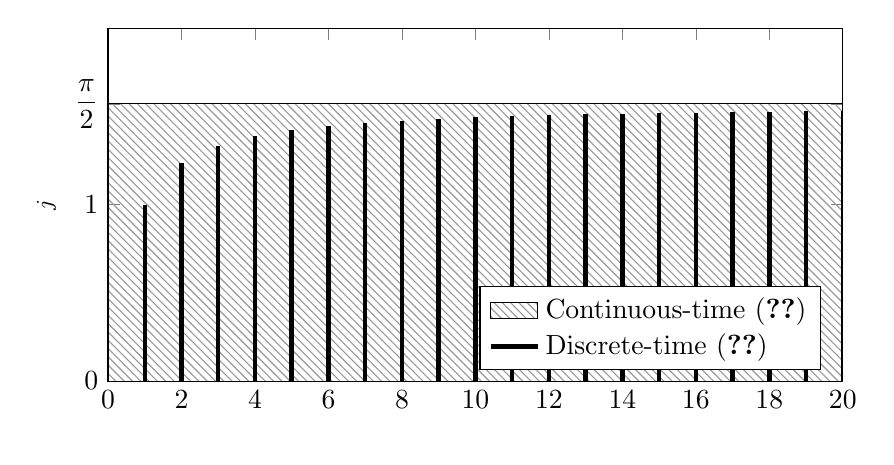
\begin{tikzpicture}[scale=1]
		\begin{axis}[xmin=0,xmax=20,ymin=0,ymax=2,
			ytick = {0,1,pi/2},yticklabels = {$ 0 $,$ 1 $,$ \dfrac{\pi}{2} $},
			tick label style={font=\normalsize},
			xlabel=$ \taun $,ylabel=$ \gpos_j\taun $,label style={font=\large},
			trig format plots=rad,
			legend pos=south east,legend style={font=\normalsize},legend cell align={left},
			width=.9\linewidth,height=.5\linewidth]
			\addplot[draw=black,pattern=north west lines,pattern color=black!40,area legend] (0,0) rectangle (20,pi/2);
			\addplot[domain=1:20,samples=20,mark=none,ycomb,ultra thick] {x*2*sin(pi/(2*(2*x+1)))};
			\addplot[draw=black,ultra thick] (20,0) -- (20,1);
			\legend{Continuous-time~\eqref{eq:cont-time-single-int-variance-condition},,Discrete-time~\eqref{eq:disc-time-single-int-stability-condition}};
		\end{axis}
	\end{tikzpicture}
	\caption{Stability regions of decoupled single integrators.}
	\label{fig:stability-region-single-int}
\end{figure}
					%!TEX ROOT = ../../centralized_vs_distributed.tex

\myParagraph{\titlecap{performance evaluation}}\label{sec:disc-time-single-int-moment-matching}
With fixed parameters,
the steady-state variance of each decoupled subsystem
can be computed numerically via the Wiener–Khintchine formula. % recalled in~\autoref{app:disc-time-single-int-variance-explicit}.
Also, for any given value of $ \taun $,
%gain-parametric 
a closed-form expression of the variance
%whose convexity can be easily assessed,
can be obtained via moment matching through a recursive formula, see~\cref{app:disc-time-single-int-variance-explicit}.
Such closed-form expressions have been used for our computational experiments illustrated in~\autoref{fig:opt-var}.
\textcolor{subsectioncolor}{Figure~\ref{fig:disc-time-var}} shows the typical profiles
of the variance function for decoupled subsystems with single- and double-integrator dynamics
(see~\eqref{eq:disc-time-single-int-decoupled} and~\eqref{eq:disc-time-double-int-decoupled} in~\cref{app:disc-time-single-int-variance-explicit},
respectively).
%For the one-dimensional case (single integrator),
%convexity of the variance function $ \var{\gpos_i} $ can be checked
%by studying the second derivative. % solving a system of inequalities.
%%over the decoupled subsystems.
%\autoref{fig:disc-time-var} shows the level curves of the variance,
%which looks convex also for the double integrator.

\begin{figure}
	\centering
	\begin{minipage}{.5\linewidth}
		\centering
		\includegraphics[width=\linewidth]{disc-time-single-int-var}
	\end{minipage}%
	\hfil
	\begin{minipage}{.5\linewidth}
		\centering
		\includegraphics[width=\linewidth]{disc-time-double-int-var-heatmap}
	\end{minipage}
	\caption{Typical profiles of the steady-state variance
		for decoupled discrete-time single integrators (left) and double integrators (right). %with $ \delayn \in \{5,7\} $.
%		The minima are highlighted by markers.
	}
	\label{fig:disc-time-var}
\end{figure}
	
\begin{comment}
\begin{figure}
\includegraphics[width=\linewidth]{figs/beyond_tss_lesion.pdf}
\caption[]{End-to-End runtime lesion study of the entire MNIST dataset and the FMA featurized music dataset. Each of DROP's contributions provides a runtime improvement.}
\label{fig:beyond_lesion}
\end{figure}
\end{comment}



\section{Conclusion}
\label{sec:conclusion}

Advanced data analytics techniques must scale to rising data volumes. 
DR techniques offer a powerful toolkit when processing these datasets, with PCA frequently outperforming popular techniques in exchange for high computational cost. 
In response, we propose DROP, a new dimensionality reduction optimizer. 
DROP combines progressive sampling, progress estimation, and online aggregation to identify high quality low dimensional bases via PCA without processing the entire dataset by balancing the runtime of downstream tasks and achieved dimensionality. 
Thus, DROP provides a first step in bridging the gap between quality and efficiency in end-to-end DR for downstream \red{analytics}. 

%We revisit canonical operators for time series dimensionality reduction and the measurement study of~\cite{keogh-study}, and show that PCA is more effective than popular alternatives in the data mining literature often by a margin of over $2\times$ on average on gold-standard time series benchmark data sets with respect to output data dimension. More surprisingly, we empirically demonstrate that a small number of samples are sufficient to accurately characterize directions of maximum variance and obtain a high-quality low-dimensional transformation.



	
	\if0\mode
	\bibliographystyle{IEEEtran}
	\bibliography{bibfile}
	\else
	\input{centralized_vs_distributed_arxiv.bbl}
	\fi
	
	\appendix
	\numberwithin{equation}{subsection}
	%!TEX ROOT = ../centralized_vs_distributed.tex

\subsection{Proof of~\cref{prop:cont-time-double-int-stability}}\label{app:cont-time-double-int-stability}

%Let us consider the following generic scalar stochastic retarded linear system driven by a standard Brownian motion:
%\begin{equation}\label{eq:2nd-order-diff-eq}
%\dfrac{d^2\x{}{t}}{dt^2} + \gvel\dfrac{d\x{}{t}}{dt} + \gvel\gpos\x{}{t-1} = \dfrac{d\noise{}{t}}{dt}
%\end{equation}
The error dynamics equation with agent model~\eqref{eq:cont-time-double-int-model} reads
\begin{equation}\label{eq:multi-agent-state-space}
	\begin{array}{c}
		d\x{}{t} =
			\left(A_0\x{}{t} + A_1\x{}{t-1}\right)dt + Bd\noisebar{}{t}, \\[10pt]
		A_0 = \begin{bmatrix}
			0 & I\\
			0 & -\gvel I
		\end{bmatrix}, \
		A_1 = \begin{bmatrix}
			0 & 0\\
			-\gvel K & 0
		\end{bmatrix}, \
		B = \begin{bmatrix}
			0\\
			I
		\end{bmatrix},
	\end{array}
\end{equation}
with $ \noisebar{}{t} $ standard $ N $-dimensional Brownian motion.
The decoupling~\eqref{eq:agent-dynamics-1}
is obtained from~\eqref{eq:multi-agent-state-space} through
the change of basis $ \x{}{t} = (T\otimes I_2)\xtilde{}{t} $.
Rewriting~\eqref{eq:agent-dynamics-1} as a double integrator in state-space form 
with state $ \tilde{s}_j(\cdot) $ yields
\begin{equation}\label{eq:2n-order-system-state-space-1}
	\begin{array}{c}
		d\tilde{s}_j(t) = \left(F_0\tilde{s}_j(t)+F_{1j}\tilde{s}_j(t-1)\right)dt + Gd\noisebar{j}{t}, \\[5pt]
		 F_0 = \begin{bmatrix}
			0 & 1\\
			0 & -\gvel
		\end{bmatrix}, \ F_{1j} = \begin{bmatrix}
			0 & 0\\
			-\gvel\gpos_j & 0
		\end{bmatrix}, \ G = \begin{bmatrix}
			0\\
			1
		\end{bmatrix},
	\end{array}
\end{equation}
Stability of~\eqref{eq:multi-agent-state-space}
is equivalent to that of~\eqref{eq:2n-order-system-state-space-1} for all $ j $.
In the following, we drop the subscript $ j $ for the sake of readability.
%The first subsystem is stable for any $ \gvel > 0 $.
For positive eigenvalues $ \gpos $,~\eqref{eq:2n-order-system-state-space-1} is mean-square asymptotically stable
if $ \alpha_0 < 0 $ and unstable if $ \alpha_0 > 0 $~\cite{wangBoundedness}, where the \emph{spectral abscissa} is defined as
\begin{equation}\label{eq:2nd-order-system-stability-condition}
	\alpha_0 \doteq \sup\left\lbrace\Re(z) : z\in \mathbb{C}, \ h(z) = 0 \right\rbrace,
\end{equation}
and the \emph{characteristic polynomial} of~\eqref{eq:2n-order-system-state-space-1} is
\begin{equation}\label{eq:2n-order-system-chacteristic-polynomial}
	\begin{aligned}
		h(z) &\doteq \det\left(zI - F_0 - F_{1}\e^{-z}\right) = z^2 + \gvel z + \gvel\gpos\e^{-z}.  % = z^2 + \gvel z + \gvel\gpos\e^{-z}
%			 &= (z^2+\gvel z)\e^{z} + \gvel\gpos
	\end{aligned}
\end{equation}
A sufficient and necessary condition for all roots of $ h(z) $ to lie in the open left-hand half-plane is derived in~\cite{BAPTISTINI1997259}.
%and rewritten below for the sake of convenience.
\begin{thm}[\!\!\protect{\cite[Theorem 2.1]{BAPTISTINI1997259}}]\label{thm:stable-roots}
	Let the 2-vectors $v(b)=\left(p b, q-b^{2}\right), w(b)=$ $(\cos b, \sin b), b \geq 0,$ be given. If $r>0,$ a necessary and sufficient condition for all roots of the equation $h(z)=(z^2+pz+q)\e^{z} + r=0$ to have negative real part is that the orthogonality condition $v(b) \cdot w(b)=0,$ with $b \in \cup_{k=0}^{\infty}(2 k \pi,(2 k+1) \pi),$ implies $|v(b)|>r$.
\end{thm}
%In virtue of the above result, 
From~\cref{thm:stable-roots},~\eqref{eq:2n-order-system-state-space-1}
is asymptotically stable if the following implication holds for $b \in \cup_{k=0}^{\infty}(2 k \pi,(2 k+1) \pi)$,
\begin{equation}\label{eq:stability-condition-1}
	\gvel b\cos b - b^2\sin b = 0 \implies \gvel^2b^2+b^4>\gvel^2\gpos^2.
\end{equation}
In view of $ b \ge 0 $ and $ \sin b \ge 0 $,~\eqref{eq:stability-condition-1}
leads to~\eqref{eq:cont-time-double-int-stability-condition} after standard algebraic manipulations,
where we replace $ b $ with $ \beta = \min b \in (0,\nicefrac{\pi}{2}) $.
The inequality can be rewritten as
\begin{equation}\label{eq:stability-condition-lambda}
	\gpos < \dfrac{\beta}{\sin\beta} \doteq \phi(\gvel),
\end{equation}
where the definition of $ \phi(\cdot) $ follows from the implicit function theorem
applied to $ F(\gvel,\beta) \doteq \beta\tan\beta - \gvel $,
which states that $ F(\gvel,\beta) = 0 $ if and only if $ \beta = \varphi(\gvel) $ and
%$ \varphi'(\cdot), \varphi''(\cdot) $ can be explicitly computed, with
\begin{equation}\label{eq:varphi-of-eta-derivative}
	\varphi'(\gvel) = \dfrac{\cos^2\left(\varphi(\gvel)\right)}{\varphi(\gvel) + \sin\left(\varphi(\gvel)\right)\cos\left(\varphi(\gvel)\right)}
\end{equation}
Tedious but straightforward calculations on the first and second derivatives %$ \phi'(\gvel) $ and $ \phi''(\gvel) $
show that $ \phi(\gvel) $ is concave increasing for any $ \gvel > 0 $.
The limits at $ 0 $ and $ +\infty $ can be easily computed
by noting that
\begin{equation}\label{eq:stability-condition-limits}
	\beta_0\doteq\varphi(0) = 0, \quad \beta_\infty\doteq\lim_{\gvel\rightarrow+\infty}\varphi(\gvel) = \dfrac{\pi}{2}.
\end{equation}





	%!TEX ROOT = ../centralized_vs_distributed.tex

\subsection{\titlecap{derivation of first-order reduced model for continuous-time double integrators}}\label{app:time-scale-separation}

We now show that subsystem~\eqref{eq:agent-dynamics-1}
can be approximated to first-order dynamics
%when the control input is sufficiently powerful.
when the gain $ \gvel $ is sufficiently high.
%We first rewrite~\eqref{eq:agent-dynamics-1} in state-space form:
%\begin{equation}\label{eq:2n-order-system-state-space}
%\begin{aligned}
%d\x{}{t} &= \z{}{t}dt\\
%d\z{}{t} &= \left(-\gvel \z{}{t} - \gvel\gpos \x{}{t-1}\right)dt + d\noise{}{t}
%\end{aligned}
%\end{equation}
Let us consider~\eqref{eq:2n-order-system-state-space-1} with state $ \tilde{s}(t) = [\xtilde{}{t},\ztilde{}{t}]^\top $.
Assume that the feedback gain $ \gvel $ is large,
so that the variable $ \ztilde{}{t} $ evolves faster than $ \xtilde{}{t} $.
We can then approximate the dynamics of $ \ztilde{}{t} $ 
by letting $ \xtilde{}{t-1} \equiv x_0 $ be constant overtime,
\begin{equation}\label{eq:z-dynamics-with-constant-x}
d\ztilde{}{t} = \left(-\gvel \ztilde{}{t} - \gvel\gpos x_0\right)dt + d\noise{}{t}.
\end{equation}
\cref{eq:z-dynamics-with-constant-x} defines a standard Ornstein–Uhlenbeck process,
\begin{equation}\label{eq:z-solution-constant-x}
\ztilde{}{t} \sim \gauss\left( \e^{-\gvel t}(\ztilde{}{0} + \gpos x_0) - \gpos x_0, \dfrac{1}{2\gvel}\left(1-\e^{-2\gvel t}\right) \right).
\end{equation}
In view of the time-scale separation,
we assume that~\eqref{eq:z-solution-constant-x} holds (with $ \xtilde{}{t-1} $ constant) till $ \ztilde{}{t} $ settles at steady state, %the limit, tends to
\begin{equation}\label{eq:z-solution-constant-x-limit-gvel}
\lim_{t \rightarrow +\infty}\ztilde{}{t} = \tilde{z}_{\infty} \sim \gauss\left( - \gpos x_0, \dfrac{1}{2\gvel} \right).
\end{equation}
Using~\eqref{eq:z-solution-constant-x-limit-gvel},
we now approximate the dynamics of $ \xtilde{}{t} $ %in~\eqref{eq:agent-dynamics-1}
as if $ \ztilde{}{t} $ reached the steady state instantaneously,
\begin{equation}\label{eq:x-dynamics-1st-order}
d\xtilde{}{t} \approx \tilde{z}_{\infty}dt = -\gpos\xtilde{}{t-1}dt + dn(t),
\end{equation}
where 
%the drift only contains the dominant term $ -\gpos\x{}{t-1} $ and
the diffusion is embedded into the Brownian noise $ n(t) $ with variance proportional to $ \nicefrac{1}{\gvel} $.
In particular, as $ \gvel \rightarrow +\infty $,
$ \tilde{z}_{\infty} \xrightarrow{a.s.} - \gpos x_0 $
and~\eqref{eq:x-dynamics-1st-order} tends to deterministic dynamics.
	%!TEX ROOT = ../centralized_vs_distributed.tex

\newpage
\subsection{\titlecap{Computation of suboptimal variance for continuous-time single integrators}}\label{app:cont-time-single-int-suboptimal-variance-computation}

%Consider the suboptimal gain $ \tilde{k}^* $ as per~\cref{prop:subopt-gain}.
The $ N $ suboptimal eigenvalues have expression (cf.~\cite{circulant})
\begin{equation}\label{eq:eigenvaluesCirculant}
	\tilde{\gpos}_j^* = 2\tilde{k}^* \left(n - \sum_{\ell=1}^n\cos\left(\dfrac{2\pi (j-1) \ell}{N}\right)\right), %, \ j=1,\dots,N
\end{equation}
which we write as $ \tilde{\gpos}_j^* = g_j(n)\tilde{k}^* $.
Being $ \tilde{k}^* = \tilde{\alpha}^*(n) \opteig $
according to~\cref{prop:subopt-gain},
we write $ \tilde{\gpos}_j^* = \tilde{c}_j^*(n)\opteig $ with $  \tilde{c}_j^*(n) \doteq g_j(n)\tilde{\alpha}^*(n) $.
Then, each subsystem~\eqref{eq:cont-time-single-int-subsystem} has variance %$ \sigma_{\textit{ss}}^{2,I}(\tilde{\gpos}_j^*) $ is
\begin{align}\label{eq:optimalVarianceLambda_i}
	\varx{\tilde{\lambda}_j^*}{I} = \dfrac{1+\sin(\tilde{\lambda}_j^* \taun)}{2\tilde{\lambda}_j^*\cos(\tilde{\lambda}_j^* \taun)}
	\overset{(i)}{=} \underbrace{\dfrac{1+\sin(\tilde{c}_j^*(n)\beta^*)}{2\tilde{c}_j^*(n)\beta^*\cos(\tilde{c}_j^*(n)\beta^*)}}_{\doteq\tilde{C}_{j}^*(n)}\taun 
%	= \tilde{C}_{j}^*(n)\taun,
%	\begin{split}
%		\varx{\tilde{\lambda}_j^*}{I} &= \dfrac{1+\sin(\tilde{\lambda}_j^* \taun)}{2\tilde{\lambda}_j^*\cos(\tilde{\lambda}_j^* \taun)} \\
%		%&= \dfrac{1+\sin(g(n)\tilde{c}^*(n)\opteig \taun)}{2g(n)\tilde{c}^*(n)\opteig\cos(g_n)\tilde{c}^*(n)\opteig \taun)} \\
%		&\overset{(i)}{=} \dfrac{1+\sin(\tilde{c}_j^*(n)\beta^*)}{2\tilde{c}_j^*(n)\beta^*\cos(\tilde{c}_j^*(n)\beta^*)}\taun = \tilde{C}_{j}^*(n)\taun,
%	\end{split}
\end{align}
where~\eqref{eq:optimal-variance-closed-form} is used in \textit{(i)}.
%$ a_i^*(n) \doteq g_i(n)\tilde{c}^*(n) $ and
%$ \tilde{C}_i^*(n) $ multiplies $ \taun $ in the third line of~\eqref{eq:optimalVarianceLambda_i}.
%The scalar variance can then be written as
%\begin{equation}\label{eq:scalarVarianceSumExplicit}
%\optvarx = \sum_{i=2}^N \tilde{C}_i^*(n)\taun = \tilde{C}^*(n)f(n)\tau_{\textit{min}}
%\end{equation}
%where $ \displaystyle \tilde{C}^*(n) \doteq \sum_{i=2}^N \tilde{C}_i^*(n) $.
	%!TEX ROOT = ../centralized_vs_distributed.tex

\subsection{\titlecap{stability conditions for discrete-time systems}}\label{app:disc-time-single-int-stability}

\begin{figure}
	\centering
	%!TEX ROOT = ../centralized_vs_distributed.tex

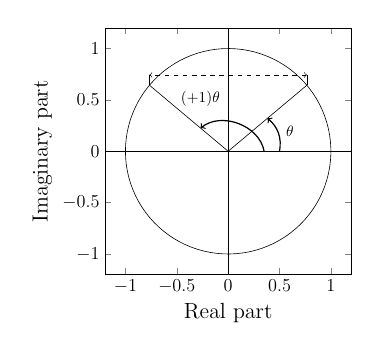
\begin{tikzpicture}[scale=.55]
	\begin{axis}[
		xlabel = Real part,
		ylabel = Imaginary part,
		axis equal image,
		ymin = -1.2,
		ymax = 1.2,
		xmin = -1.2,
		xmax = 1.2]
		\addplot [domain=-180:180, samples=100] ({cos(x)},{sin(x)});
		\draw (-1.2,0) -- (1.2,0);
		\draw (0,-1.2) -- (0,1.2);
		\draw (0,0) -- ({cos(40)},{sin(40)});
		\draw (0,0) -- ({-cos(40)},{sin(40)});
		\path[->,thick] (.5,0) edge[bend right] node [left] {}  ({.5*cos(40)},{.5*sin(40)});
		\path[->,thick] (.35,0) edge[bend right=60] node [left] {}  ({-.35*cos(40)},{.35*sin(40)}) ;
		\node at (.6,.2) {$ \delayn \theta $};
		\node at (-.27,.51) {$ (\delayn+1) \theta $};	
		\draw[<->,dashed] ({cos(40)},{sin(40)+.1}) -- ({-cos(40)},{sin(40)+.1});
		\draw ({cos(40)},{sin(40)+.1}) -- ({cos(40)},{sin(40)});
		\draw (-{cos(40)},{sin(40)+.1}) -- (-{cos(40)},{sin(40)});
		\node at (0.05,{sin(40)+.2}) {$ \gpos $};
	\end{axis}
\end{tikzpicture}
	\caption{A solution of~\eqref{eq:disc-time-single-int-uint-poles-system} in the complex plane.}
	\label{fig:disc-time-single-int-unit-poles}
\end{figure}

\myParagraph{\titlecap{General case}}
In the following, we replace $ \taun $ with $ \delayn $ % drop the subscript from $ \taun $
for the sake of readability.
For the single-integrator case, decoupling the error dynamics yields scalar subsystems of the form
\begin{equation}\label{eq:disc-time-single-int-decoupled}
	\xtilde{}{k+1} = \xtilde{}{k} - \gpos\xtilde{}{k-\tau} + \noisetilde{}{k}.
\end{equation}
The characteristic polynomial $ h(z) $ of~\eqref{eq:disc-time-single-int-decoupled} is obtained by
applying the lag operator $ z $
such that $ \xtilde{}{k}h(z) = \noisetilde{}{k} $,
\begin{equation}\label{eq:disc-time-single-int-characteristic-polinomial}
	h(z) = z - 1 + \gpos z^{-\tau}.
\end{equation}
Similarly, the double-integrator decoupled subsystems are
\begin{equation}\label{eq:disc-time-double-int-decoupled}
%	\xtilde{i}{k+1} = (2-\gvel)\xtilde{i}{k} - (1-\gvel)\xtilde{i}{k-1} - \gvel\gpos\xtilde{i}{k-\taun-1} + \noisetilde{i}{k}
	\begin{aligned}
		\xtilde{}{k+1} &= \xtilde{}{k} + \ztilde{}{k}\\
		\ztilde{}{k+1} &= (1-\gvel)\ztilde{}{k} - \gvel\gpos\xtilde{}{k-\tau} + \noisetilde{}{k},
	\end{aligned}
\end{equation}
with characteristic polynomial
\begin{equation}\label{eq:disc-time-double-int-characteristic-polinomial}
	h(z) = z-2+\gvel+(1-\gvel)z^{-1}+\gvel\gpos z^{-\tau-1}.
\end{equation}
For positive $ \gpos $, stability of~\eqref{eq:disc-time-single-int-decoupled}--\eqref{eq:disc-time-double-int-decoupled}
can be assessed via the Jury stability criterion,
which provides necessary and sufficient conditions for
the roots of~\eqref{eq:disc-time-single-int-characteristic-polinomial} and~\eqref{eq:disc-time-double-int-characteristic-polinomial}
to lie inside the unit circle %in the complex plane
in the form of inequalities involving the coefficients of $ h(z) $.
Being the latter polynomial in $ \gvel $ and $ \gpos $,
the Jury criterion %applied to~\eqref{eq:disc-time-single-int-model}--\eqref{eq:disc-time-double-int-model}
yields $ \Theta(N\tau) $ polynomial inequalities in the feedback gains,
which can be computed through standard software tools.

\myParagraph{Proof of~\cref{prop:disc-time-single-int-stability}}
\cref{eq:disc-time-single-int-characteristic-polinomial} can be studied as a root locus
by varying the gain $ \gpos $.
In particular, $ \gpos = 0 $ yields
a multiple root at $ z_1^* = 0 $ and a simple root at $ z_2^* = 1 $.
Negative values of $ \gpos $ are discarded as they push the latter outside the unit circle.
As $ \gpos $ increases,
the branches leave the unit ball along their asymptotes.
%Notice that, in view of the structure of the root locus,
The admissible values for $ \gpos $ are upper bounded by a threshold gain $ \gpos_{\textit{th}} $
beyond which some roots leave the unit ball.
In particular, we are interested in the minimum gain for which at least one root lies exactly on the unit circle.
Thus, we are looking for roots of~\eqref{eq:disc-time-single-int-characteristic-polinomial}
of the form $ z = \e^{j\theta} $,
\begin{equation}\label{eq:disc-time-single-int-unit-poles-eq}
	\e^{j(\delayn+1)\theta} - \e^{j\delayn\theta} + \gpos = 0.
\end{equation}
\cref{eq:disc-time-single-int-unit-poles-eq} can be equivalently written as the system
\begin{equation}\label{eq:disc-time-single-int-uint-poles-system}
	\begin{cases}
		\cos((\delayn+1)\theta) - \cos(\delayn\theta) + \gpos = 0\\
		\sin((\delayn+1)\theta) = \sin(\delayn\theta).
	\end{cases}
\end{equation}
\autoref{fig:disc-time-single-int-unit-poles} depicts a solution of~\eqref{eq:disc-time-single-int-uint-poles-system} for $ \sin(\delayn\theta) > 0 $.
The case $ \sin(\delayn\theta)<0 $ is analogous
and is omitted.
Further, the solution $ (\delayn+1)\theta = \delayn\theta $
can be discarded because it implies $ \gpos = 0 $ and thus prevents asymptotic stability.
%On the other hand, 
%Therefore, we only focus on the case $ \sin(\delayn\theta)>0 $. % depicted in the left box in~\autoref{fig:disc-time-single-int-unit-poles}.
From basic trigonometric arguments (c.f.~\autoref{fig:disc-time-single-int-unit-poles}),
the second equation in~\eqref{eq:disc-time-single-int-uint-poles-system} implies
\begin{equation}\label{eq:disc-time-single-int-theta}
	\delayn\theta + \dfrac{\theta}{2} = \dfrac{\pi}{2} + 2k\pi \ \longrightarrow \ \theta = \dfrac{\pi+4k\pi}{2\delayn+1}, \quad 
\end{equation}
where we impose $ \theta \in [0,\pi] $
and thus $ k\in\{0,\dots,\floor{\nicefrac{\delayn}{2}}\} $.
This includes all possible cases,
because the roots of~\eqref{eq:disc-time-single-int-characteristic-polinomial} come in complex conjugates pairs.
From~\eqref{eq:disc-time-single-int-theta},
the first equation in~\eqref{eq:disc-time-single-int-uint-poles-system},
and the fact $ \cos((\delayn+1)\theta) = - \cos(\delayn\theta) $,
we retrieve
\begin{equation}\label{eq:disc-time-single-int-unit-roots-gain}
	\gpos = 2\cos\left(\dfrac{\pi\delayn+4k\pi\delayn}{2\delayn+1}\right).
\end{equation}
The right-hand term in~\eqref{eq:disc-time-single-int-unit-roots-gain} is monotone increasing in $ k $.
Indeed, taking the argument of the cosine modulus $ 2\pi $ yields
\begin{equation}\label{eq:disc-time-single-int-angle-modulus}
	\dfrac{\pi\delayn+4k\pi\delayn}{2\delayn+1} \ \mod \ 2\pi = \dfrac{\pi\delayn-2k\pi}{2\delayn+1} \in \left[0,\dfrac{\pi}{2}\right),
\end{equation}
which is nonnegative and monotone decreasing in $ k $ for any $ \tau $.
Finally, the upper bound for the gain $ \gpos $ is given by
\begin{equation}\label{eq:disc-time-single-int-threshold-gain}
	\gpos_{\textit{th}} = \min_k2\cos\left(\dfrac{\pi\delayn+4k\pi\delayn}{2\delayn+1}\right) = 2\cos\left(\dfrac{\pi\delayn}{2\delayn+1}\right).
% 2\sin\left(\dfrac{\pi}{2}\dfrac{1}{2\delayn+1}\right)
\end{equation}



	\if0\mode
	%!TEX ROOT = ../centralized_vs_distributed.tex

\subsection{\titlecap{variance computation for discrete-time systems}}\label{app:disc-time-single-int-variance-explicit}

\myParagraph{Wiener--Kintchine Formula}
Given any fixed values of delay and feedback gains,
the steady-state variance $ \varx{\gpos}{I} $ or $ \varx{\gvel,\gpos}{II} $ of the decoupled subsystems can be computed numerically by
\begin{equation}\label{eq:disc-time-variance-integral}
	\dfrac{1}{2\pi}\int_{-\pi}^{+\pi}\dfrac{d\theta}{|h(\e^{j\theta})|^2},
\end{equation}
where the characteristic polynomial $ h(z) $
is~\eqref{eq:disc-time-single-int-characteristic-polinomial} or~\eqref{eq:disc-time-double-int-characteristic-polinomial}.

\myParagraph{Single Integrator Model}
The moment-matching method applied to subsystem~\eqref{eq:disc-time-single-int-decoupled} yields 
a linear system of equations in the variables $ (\rho_0,...,\rho_\delayn) $,
where $ \rho_t \doteq \mathbb{E}[\xtilde{}{k}\xtilde{}{k\pm t}] $:
\begin{subequations}\label{eq:disc-time-single-int-moment-matching-eqs}
	\begin{align}
		\rho_0 &= \mathbb{E}[\xtilde{}{k+1}^2] = \rho_0 + \gpos^2\rho_0 + 1 - 2\gpos\rho_\delayn \label{eq:disc-time-single-int-first-moment-eq}\\
		\rho_1 &= \mathbb{E}[\xtilde{}{k+1}\xtilde{}{k}] = \rho_0 - \gpos\rho_\delayn \label{eq:disc-time-single-int-yule-walker-eqs-1}\\
		&\hspace{2mm}\vdots \nonumber \\
		\rho_\delayn &= \rho_{\delayn-1} - \gpos\rho_1, \label{eq:disc-time-single-int-yule-walker-eqs-2}
	\end{align}
\end{subequations}
where~\eqref{eq:disc-time-single-int-yule-walker-eqs-1}--\eqref{eq:disc-time-single-int-yule-walker-eqs-2} are the Yule-Walker equations.
%associated to the decoupled subsystem~\eqref{eq:disc-time-single-int-decoupled}.
System~\eqref{eq:disc-time-single-int-moment-matching-eqs}
can be written compactly as $ A^{(\tau)}\rho = e_1 $, 
where $ \rho^\top = [\rho_0,\dots,\rho_{\delayn}]$,
$ e_1 $ is the canonical vector in $ \Real{\delayn+1} $ with nonzero first coordinate,
and $ A^{(\tau)}\in\Real{(\delayn+1)\times(\delayn+1)} $ gathers all coefficients of equations in~\eqref{eq:disc-time-single-int-moment-matching-eqs}.
%with
%\begin{equation}\label{eq:explicit-variance-matrix-A}
%A^{(\tau)} = \begin{bmatrix}
%-\gpos^2 &   		&     		& 		 &   	  & 2\gpos\\
%1 		 & -1 		&     		& 		 &    	  & -\gpos\\
%& 	\ddots	& \ddots	&  		 & \iddots&  \\
%& 			& 			&		 & 		  &  \\
%& 			& 			&		 & 		  &  \\
%& -\gpos	& 			& 		 & 1 	  & -1
%\end{bmatrix}.
%\end{equation}
%In particular, when $ \delayn $ is odd, the $ (\ceil{\nicefrac{\delayn}{2}} + 1) $-th row is
%\begin{equation}\label{eq:app-explicit-variance-matrix-A-mid-row-odd}
%	\left[\!\begin{array}{cccccccc}
%	0 & \dots & 0 & 1 & -1-\gpos & 0 & \dots & 0
%	\end{array}\!\right],
%\end{equation}
%while, when $ \delayn $ is even, the $ (\nicefrac{\delayn}{2} + 2) $-th row is
%\begin{equation}\label{eq:app-explicit-variance-matrix-A-mid-row-even}
%	\left[\!\begin{array}{cccccccc}
%		0 & \dots & 0 & 1-\gpos & -1 & 0 & \dots & 0
%	\end{array}\!\right].
%\end{equation}
%where we highlight the dependence on the delay in view of the recursive characterization of $ \rho_0 $.
It can be seen that $ A^{(\tau)} $ is full rank for all $ \delayn \ge 1 $ and thus~\eqref{eq:disc-time-single-int-moment-matching-eqs} has a unique solution.
In particular, we are interested in the autocorrelation $ \rho_0 = \varx{\gpos}{I} $,
which is given by
the ratio between the minor associated with the top-left element of $ A^{(\tau)} $,
named $ n_\delayn \doteq M^{(\tau)}_{1,1} $, and the determinant $ d_\delayn \doteq \det(A^{(\tau)}) $.
Specifically, $ \rho_0 $ is a rational function in $ \gpos $
and can be computed in closed form by a symbolic solver
given any value of $ \delayn $.

Further, $ n_{\delayn} $ and $ d_{\delayn} $ can be explicitly computed %recursively via an inductive argument on the delay $ \delayn $, 
by leveraging a recursive nested structure of the matrix $ A $.
%\begin{equation}\label{eq:recursive-matrix}
%	A^{(\delayn)} = \tikz[baseline=(M.west)]{%
%		\node[matrix of math nodes,matrix anchor=west,left delimiter={[},right delimiter={]},ampersand replacement=\&] (M) {%
%		-\gpos^2\&			\&			\&							\& 							\&						 \&	-2\gpos		\\
%			1 	\& -1  		\&    		\&							\& 							\& 						 \&	  			\\
%				\&  1  		\&  -1		\&	  						\&      					\& 						 \& -\gpos   	\\
%				\&    		\&   1 		\& \textcolor{white}{t1}	\& 							\& 						 \&				\\
%				\&			\&			\&							\& \tilde{A}^{(\delayn-4)}	\&						 \&				\\
%				\& 			\&	  		\& 							\&	 						\& \textcolor{white}{t1} \&				\\
%				\& 		    \&   -\gpos	\&							\&							\& 1					 \&	-1			\\
%				\& 	-\gpos	\&	  		\&							\&							\&						 \&	1			\\			
%		};
%		\node[draw,fit=(M-3-3)(M-7-7),inner sep=-1pt] {};
%		\node[draw,fit=(M-4-4)(M-6-6),inner sep=-1pt] {};
%	}.
%\end{equation}
%where $ \tilde{A}^{(\delayn)} $ is the submatrix of $ A^{(\delayn)} $ obtained by removing its first row and column
%such that $ M^{(\delayn)}_{1,1} = \det(\tilde{A}^{(\delayn)}) $,
%and the matrices $ \tilde{A}^{(\delayn-2)} $ and $ \tilde{A}^{(\delayn-4)} $ are framed in~\eqref{eq:recursive-matrix}.
The solution obeys the following recursive expression in $ \delayn $:
%\begin{prop}\label{prop:disc-time-single-int-variance-explicit}
\begin{subequations}\label{eq:disc-time-single-int-variance-explicit}
	\begin{gather}
		n_\delayn = \begin{dcases}
			(-1-\gpos)n_{\delayn-1} + \tilde{n}_{\delayn-1} & \mbox{if } \delayn \mbox{ odd}\\
			-(1-\gpos)n_{\delayn-1} - \gpos\tilde{n}_{\delayn-1} & \mbox{if }\delayn \mbox{ even},\\
		\end{dcases} \label{eq:disc-time-single-int-variance-explicit-numerator}\\
		\tilde{n}_{\delayn} = (2-\gpos^2)\tilde{n}_{\delayn-2} - \tilde{n}_{\delayn-4}, \label{eq:disc-time-single-int-variance-explicit-numerator-rem}\\
		d_\delayn = d_{\delayn-2} - \gpos^2\left(n_\delayn+n_{\delayn-2}\right), \label{eq:disc-time-single-int-variance-explicit-denominator}\\
		\tilde{n}_{-3} = -1+\gpos^2, \ \tilde{n}_{-2} = \gpos^2, \ \tilde{n}_{-1} = -1, \ \tilde{n}_0 = 0, \\
		n_{-1} = 0, \ n_0 = 1, \ d_{-1} = -2\gpos, \ d_0 = 2\gpos-\gpos^2.
	\end{gather}
\end{subequations}
Detailed derivation of~\eqref{eq:disc-time-single-int-variance-explicit}
is given in the technical report~\cite{2021arXiv210900359B}.
Given $ \delayn $,
convexity of $ \rho_0 $ in $ \gpos $ can be assessed by checking the sign
of the second derivative in the stability region.
This reduces to a system of inequalities
which can be solved, \eg by \texttt{solve\_rational\_inequalities} in Python.
The variance was proved strictly convex for all tried delays.

\myParagraph{\titlecap{double integrator model}}
System~\eqref{eq:disc-time-double-int-decoupled} yields the following
$ \delayn+2 $ coupled moment-matching equations,
%The moment-matching system associated with~\eqref{eq:disc-time-double-int-decoupled}
%has $ \delayn+2 $ variables $ (\rho_0,\dots,\rho_{\delayn+1}) $ and is composed of the following equations:
\begin{subequations}\label{eq:disc-time-double-int-moment-matching-eqs}
	\begin{align}
		\begin{split}
			\rho_0 &= [(2-\gvel)^2 + (1-\gvel)^2 + \gvel^2\gpos^2]\rho_0 - 2(2-\gvel)(1-\gvel)\rho_1 \\
			& + 2(1-\gvel)\gvel\gpos\rho_\delayn - 2(2-\gvel)\gvel\gpos\rho_{\delayn+1} + 1 \label{eq:disc-time-double-int-first-moment-eq}
		\end{split}\\
		\rho_1 &= (2-\gvel)\rho_0 - (1-\gvel)\rho_1 - \gvel\gpos\rho_{\delayn+1} \label{eq:disc-time-double-int-yule-walker-eqs-1}\\
		&\hspace{2mm}\vdots \nonumber \\
		\rho_{\delayn+1} &= (2-\gvel)\rho_\delayn - (1-\gvel)\rho_{\delayn-1} - \gvel\gpos\rho_1, \label{eq:disc-time-double-int-yule-walker-eqs-2}
	\end{align}
\end{subequations}
with~\eqref{eq:disc-time-double-int-yule-walker-eqs-1}--\eqref{eq:disc-time-double-int-yule-walker-eqs-2} the associated Yule-Walker equations.
%associated with~\eqref{eq:disc-time-double-int-decoupled}.
Analogous analysis to single-integrator model can be performed.
	\else
	%!TEX ROOT = ../centralized_vs_distributed.tex

\subsection{\titlecap{variance computation for discrete-time systems}}\label{app:disc-time-single-int-variance-explicit}

\myParagraph{Wiener--Kintchine Formula}
Given any fixed values of delay and feedback gains,
the steady-state variance $ \varx{\gpos}{I} $ or $ \varx{\gvel,\gpos}{II} $ of the decoupled subsystems can be computed numerically by
\begin{equation}\label{eq:disc-time-variance-integral}
	\dfrac{1}{2\pi}\int_{-\pi}^{+\pi}\dfrac{d\theta}{|h(\e^{j\theta})|^2},
\end{equation}
where the characteristic polynomial $ h(z) $
is~\eqref{eq:disc-time-single-int-characteristic-polinomial} or~\eqref{eq:disc-time-double-int-characteristic-polinomial}.

\myParagraph{\titlecap{single integrator model}}
The moment-matching method applied to the subsystem~\eqref{eq:disc-time-single-int-decoupled} yields 
a linear system of equations in the variables $ (\rho_0,...,\rho_\delayn) $,
where $ \rho_t \doteq \mathbb{E}[\xtilde{}{k}\xtilde{}{k\pm t}] $:
\begin{subequations}\label{eq:disc-time-single-int-moment-matching-eqs}
	\begin{align}
		\rho_0 &= \mathbb{E}[\xtilde{}{k+1}^2] = \rho_0 + \gpos^2\rho_0 + 1 - 2\gpos\rho_\delayn \label{eq:disc-time-single-int-first-moment-eq}\\
		\rho_1 &= \mathbb{E}[\xtilde{}{k+1}\xtilde{}{k}] = \rho_0 - \gpos\rho_\delayn \label{eq:disc-time-single-int-yule-walker-eqs-1}\\
		&\hspace{2mm}\vdots \nonumber \\
		\rho_\delayn &= \rho_{\delayn-1} - \gpos\rho_1, \label{eq:disc-time-single-int-yule-walker-eqs-2}
	\end{align}
\end{subequations}
where~\eqref{eq:disc-time-single-int-yule-walker-eqs-1}--\eqref{eq:disc-time-single-int-yule-walker-eqs-2} are the Yule-Walker equations.
%associated to the decoupled subsystem~\eqref{eq:disc-time-single-int-decoupled}.
System~\eqref{eq:disc-time-single-int-moment-matching-eqs}
can be written compactly as $ A^{(\tau)}\rho = e_1 $, where
$ \rho^\top = [\rho_0,\dots,\rho_{\delayn}]$,
$ e_1 $ is the canonical vector in $ \Real{\delayn+1} $ with nonzero first coordinate and $ A^{(\tau)}\in\Real{(\delayn+1)\times(\delayn+1)} $ with
\begin{equation}\label{eq:explicit-variance-matrix-A}
	A^{(\tau)} = \begin{bmatrix}
		-\gpos^2 &   		&     		& 		 &   	  & 2\gpos\\
		1 		 & -1 		&     		& 		 &    	  & -\gpos\\
		& 	\ddots	& \ddots	&  		 & \iddots&  \\
		& 			& 			&		 & 		  &  \\
		& 			& 			&		 & 		  &  \\
		& -\gpos	& 			& 		 & 1 	  & -1
	\end{bmatrix}.
\end{equation}
In particular, when $ \delayn $ is odd, the $ (\ceil{\nicefrac{\delayn}{2}} + 1) $-th row is
\begin{equation}\label{eq:app-explicit-variance-matrix-A-mid-row-odd}
	\left[\!\begin{array}{cccccccc}
		0 & \dots & 0 & 1 & -1-\gpos & 0 & \dots & 0
	\end{array}\!\right],
\end{equation}
while, when $ \delayn $ is even, the $ (\nicefrac{\delayn}{2} + 2) $-th row is
\begin{equation}\label{eq:app-explicit-variance-matrix-A-mid-row-even}
	\left[\!\begin{array}{cccccccc}
		0 & \dots & 0 & 1-\gpos & -1 & 0 & \dots & 0
	\end{array}\!\right].
\end{equation}
%where we highlight the dependence on the delay in view of the recursive characterization of $ \rho_0 $.
Notice that $ A^{(\tau)} $ is full rank for all $ \delayn \ge 1 $ and thus~\eqref{eq:disc-time-single-int-moment-matching-eqs} can be solved uniquely.
In particular, we are interested in the autocorrelation $ \rho_0 = \varx{\gpos}{I} $,
which is given by
the ratio between the minor associated with the top-left element of $ A^{(\tau)} $,
named $ n_\delayn \doteq M^{(\tau)}_{1,1} $, and the determinant $ d_\delayn \doteq \det(A^{(\tau)}) $.
Specifically, $ \rho_0 $ is a rational function in $ \gpos $
and can be computed in closed form by a symbolic solver
given any value of $ \delayn $.

Further, $ n_{\delayn} $ and $ d_{\delayn} $ can be computed %recursively via an inductive argument on the delay $ \delayn $, 
by leveraging the following nested structure of the matrix $ A^{(\delayn)} $:
\begin{equation}\label{eq:recursive-matrix}
	A^{(\delayn)} = \tikz[baseline=(M.west)]{%
		\node[matrix of math nodes,matrix anchor=west,left delimiter={[},right delimiter={]},ampersand replacement=\&] (M) {%
			-\gpos^2\&			\&			\&							\& 							\&						 \&	-2\gpos		\\
			1 	\& -1  		\&    		\&							\& 							\& 						 \&	  			\\
			\&  1  		\&  -1		\&	  						\&      					\& 						 \& -\gpos   	\\
			\&    		\&   1 		\& \textcolor{white}{t1}	\& 							\& 						 \&				\\
			\&			\&			\&							\& \tilde{A}^{(\delayn-4)}	\&						 \&				\\
			\& 			\&	  		\& 							\&	 						\& \textcolor{white}{t1} \&				\\
			\& 		    \&   -\gpos	\&							\&							\& 1					 \&	-1			\\
			\& 	-\gpos	\&	  		\&							\&							\&						 \&	1			\\			
		};
		\node[draw,fit=(M-3-3)(M-7-7),inner sep=-1pt] {};
		\node[draw,fit=(M-4-4)(M-6-6),inner sep=-1pt] {};
	},
\end{equation}
where $ \tilde{A}^{(\delayn)} $ is the submatrix of $ A^{(\delayn)} $ obtained by removing its first row and column
such that $ M^{(\delayn)}_{1,1} = \det(\tilde{A}^{(\delayn)}) $,
and the matrices $ \tilde{A}^{(\delayn-2)} $ and $ \tilde{A}^{(\delayn-4)} $ are framed in~\eqref{eq:recursive-matrix}.

The solution obeys the following recursive expression in $ \delayn $:
%\begin{prop}\label{prop:disc-time-single-int-variance-explicit}
\begin{subequations}\label{eq:disc-time-single-int-variance-explicit}
	\begin{gather}
		n_\delayn = \begin{dcases}
			(-1-\gpos)n_{\delayn-1} + \tilde{n}_{\delayn-1} & \mbox{if } \delayn \mbox{ odd}\\
			-(1-\gpos)n_{\delayn-1} - \gpos\tilde{n}_{\delayn-1} & \mbox{if }\delayn \mbox{ even},\\
		\end{dcases} \label{eq:disc-time-single-int-variance-explicit-numerator}\\
		\tilde{n}_{\delayn} = (2-\gpos^2)\tilde{n}_{\delayn-2} - \tilde{n}_{\delayn-4}, \label{eq:disc-time-single-int-variance-explicit-numerator-rem}\\
		d_\delayn = d_{\delayn-2} - \gpos^2\left(n_\delayn+n_{\delayn-2}\right), \label{eq:disc-time-single-int-variance-explicit-denominator}\\
		\tilde{n}_{-3} = -1+\gpos^2, \ \tilde{n}_{-2} = \gpos^2, \ \tilde{n}_{-1} = -1, \ \tilde{n}_0 = 0, \\
		n_{-1} = 0, \ n_0 = 1, \ d_{-1} = -2\gpos, \ d_0 = 2\gpos-\gpos^2.
	\end{gather}
\end{subequations}

\cref{eq:disc-time-single-int-variance-explicit} can be proved by an inductive argument
on the delay $ \delayn $.

\myParagraph{Numerator}
We demonstrate the formula for odd delays $ \delayn = 2k+1, k\in\mathbb{N} $.
The other case can be obtained similarly and is thus omitted. % in the interest of space.\\

Let us consider the submatrix $ \tilde{A}^{(\delayn)} \in\Real{\delayn\times\delayn} $
obtained by removing the first row and column of $ A $,
such that $ n_\delayn = \det(\tilde{A}^{(\delayn)}) $.
Replacing the $ (\floor{\nicefrac{\delayn}{2}}) $-th column with the sum of
$ (\floor{\nicefrac{\delayn}{2}}) $-th and $ (\ceil{\nicefrac{\delayn}{2}}) $-th columns yields
\begin{equation}\label{eq:numerator-1}
	\det\left(\tilde{A}^{(\delayn)}\right) = \left|\begin{array}{c|c|c}
		\tilde{A}_{11}^{(\delayn-1)} &  & \tilde{A}_{12}^{(\delayn-1)} \\
		\hline
		\begin{array}{ccc} \dots & 0 & -\gpos \end{array} & -1-\gpos & \\
		\hline
		\tilde{A}_{21}^{(\delayn-1)} & \begin{array}{c} 1 \\ 0 \\ \vdots \end{array} & \tilde{A}_{22}^{(\delayn-1)}
	\end{array}\right|,
\end{equation}
from which it follows $ n_\delayn = (-1-\gpos)n_{\delayn-1} - \det(R^{(\delayn)}) $ where $ R^{(\delayn)}\in\Real{(\delayn-1)\times(\delayn-1)} $
and the base case is $ n_1 = -1-\gpos $.
This expression corresponds to~\eqref{eq:disc-time-single-int-variance-explicit-numerator} with $ \tilde{n}_{\delayn-1} = -\det(R^{(\delayn)}) $.
Manipulations of the second term yield a further recursive expression for $ \tilde{n}_{\delayn-1} $.
Let us write
\begin{equation}\label{eq:numerator-2}
	\det\left(R^{(\delayn)}\right) =	\tikz[baseline=(M.west)]{%
		\node[matrix of math nodes,matrix anchor=west,left delimiter=|,right delimiter=|,ampersand replacement=\&] (M) {%
			-1 		\&    		\& 	  \& 	 			\& 				\&   		\& -\gpos\\
			1 		\& -1  		\&    \& 				\&  			\& -\gpos 	\&  \\
			\&  1  		\&  \textcolor{white}{t1}  \&       			\&    			\& 			\& \\
			\&    		\&    \& R^{(\delayn-4)}	\&	  			\& 			\& \\
			\& 			\&	  \&	 			\&	\textcolor{white}{t2}			\&			\&	\\
			\& \gpos    \&    \&				\&		1		\&	-1		\&	\\
			-\gpos	\& 			\&	  \&				\&				\& 	1		\& -1\\			
		};
		\node[draw,fit=(M-2-2)(M-6-6),inner sep=-1pt] {};
		\node[draw,fit=(M-3-3)(M-5-5),inner sep=-1pt] {};
	},
\end{equation}
where the two inner boxes highlight $ R^{(\delayn-2)} $ and $ R^{(\delayn-4)} $, respectively.
Straightforward calculations yield
\begin{multline}\label{eq:numerator-3}
	\det\left(R^{(\delayn)}\right) = \det\left(R^{(\delayn-2)}\right) + \\
	\gpos\tikz[baseline=(M.west)]{%
		\node[matrix of math nodes,matrix anchor=west,left delimiter=|,right delimiter=|,ampersand replacement=\&] (M) {%
			1 			\& -1  		\&    						\& 					\&  						\& -\gpos 	 \\
			\&  1  		\&  \textcolor{white}{t1}  	\&       			\&    						\& 			 \\
			\&    		\&    						\& R^{(\delayn-4)}	\&	  						\& 			 \\
			\& 			\&	  						\&	 				\&	\textcolor{white}{t2}	\&			 \\
			\& -\gpos   \&    						\&					\&		1					\&	-1		 \\
			-\gpos		\& 			\&	  						\&					\&							\& 	1		 \\			
		};
		\node[draw,fit=(M-1-2)(M-5-6),inner sep=-1pt] {};
		\node[draw,fit=(M-2-3)(M-4-5),inner sep=-1pt] {};
	}.
\end{multline}
The determinant in the second addend is computed as
\begin{equation}\label{eq:numerator-4}
	-\gpos\det\left(R^{(\delayn-2)}\right) + 
	\tikz[baseline=(M.west)]{%
		\node[matrix of math nodes,matrix anchor=west,left delimiter=|,right delimiter=|,ampersand replacement=\&] (M) {%
			1  		 \&  \textcolor{white}{t1}  \&       			\&    						\\
			\&    						\& R^{(\delayn-4)}	\&	  						\\
			\&	  						\&	 				\&	\textcolor{white}{t2}	\\
			-\gpos   \&    						\&					\&		1					\\
		};
		\node[draw,fit=(M-1-2)(M-3-4),inner sep=-1pt] {};
	},
\end{equation}
and the second addend in the above equation has the same structure as
the determinant in the second addend in~\eqref{eq:numerator-3}.
Thus, an easy inductive argument proves
\begin{multline}\label{eq:numerator-rem-recursive}
	\det\left(R^{(\delayn)}\right) = \det\left(R^{(\delayn-2)}\right) + \gpos\left(-\gpos\det\left(R^{(\delayn-2)}\right)\right.\\
	\left.-\gpos\det\left(R^{(\delayn-4)}\right) - \dots - \gpos\det\left(R^{(3)}\right)- \gpos\right),
\end{multline}
where the base case is $ \det\left(R^{(3)}\right) = -\gpos^2 $.
\cref{eq:disc-time-single-int-variance-explicit-numerator-rem} is retrieved by noting
\begin{multline}\label{eq:numerator-rem-recursive-1}
	\det\left(R^{(\delayn-2)}\right) - \left(1-\gpos^2\right)\det\left(R^{(\delayn-4)}\right) = \\
	\gpos\left(-\gpos\det\left(R^{(\delayn-6)}\right) - \dots -\gpos\right),
\end{multline}
and thus the tail of the infinite summation in~\eqref{eq:numerator-rem-recursive} can be replaced
by the left-hand term in~\eqref{eq:numerator-rem-recursive-1}.

\myParagraph{Denominator}
The denominator of $ \rho_0 $ is computed as the determinant of $ A $.
Let $ A^{(\delayn)} \doteq A $, from~\eqref{eq:explicit-variance-matrix-A} we get
\begin{multline}\label{eq:denominator-1}
	\det\left(A^{(\delayn)}\right) = -\gpos^2M_{1,1}^{(\delayn)} -\\
	2\gpos\tikz[baseline=(M.west)]{%
		\node[matrix of math nodes,matrix anchor=west,left delimiter=|,right delimiter=|,ampersand replacement=\&] (M) {%
			1 	\& -1  		\&    		\&							\& 							\& 						 \&	  			\\
			\&  1  		\&  -1		\&	  						\&      					\& 						 \& -\gpos   	\\
			\&    		\&   1 		\& \textcolor{white}{t1}	\& 							\& 						 \&				\\
			\&			\&			\&							\& \tilde{A}^{(\delayn-4)}	\&						 \&				\\
			\& 			\&	  		\& 							\&	 						\& \textcolor{white}{t1} \&				\\
			\& 		    \&   -\gpos	\&							\&							\& 1					 \&	-1			\\
			\& 	-\gpos	\&	  		\&							\&							\&						 \&	1			\\			
		};
		\node[draw,fit=(M-2-3)(M-6-7),inner sep=-1pt] {};
		\node[draw,fit=(M-3-4)(M-5-6),inner sep=-1pt] {};
	},
\end{multline}
where $ \tilde{A}^{(\delayn-2)} $ and $ \tilde{A}^{(\delayn-4)} $ are framed in the second addend above.
The latter can be computed as the following sum,
\begin{equation}\label{eq:denominator-2}
	\gpos M_{1,1}^{(\delayn-2)} + \tikz[baseline=(M.west)]{%
		\node[matrix of math nodes,matrix anchor=west,left delimiter=|,right delimiter=|,ampersand replacement=\&] (M) {%
			1  		\&  -1				\&	  						\&      								\& 							\\
			\&   1 				\& \textcolor{white}{t1}	\& 										\&							\\
			\&					\&							\& \tilde{A}^{(\delayn-4)}				\&							\\
			\&	  				\& 							\&	 									\& 	\textcolor{white}{t1}	\\
			\&   -\gpos			\&							\&										\& 1						\\
		};
		\node[draw,fit=(M-2-3)(M-4-5),inner sep=-1pt] {};
	},
\end{equation}
where the same structure is repeated recursively in the second addend above.
Thus, an easy inductive argument proves
\begin{equation}\label{eq:denominator-recursirve}
	d_\delayn = -\gpos^2n_\delayn - 2\gpos\left(\gpos n_{\delayn-2} + \gpos n_{\delayn-4} + \dots + \gpos n_1 + 1\right),
\end{equation}
where the base case is $ d_1 = -\gpos^2(-1-\gpos)-2\gpos $.
\cref{eq:disc-time-single-int-variance-explicit-denominator} is retrieved by noting
\begin{multline}\label{eq:denominator-recursirve-1}
	-2\gpos\left(\gpos n_{\delayn-2} + \gpos n_{\delayn-4} + \dots + 1\right) = \\
	-\gpos^2 n_{\delayn-2} -\gpos^2 n_{\delayn-2} - 2\gpos\left(\gpos n_{\delayn-4} + \dots + 1\right) = \\
	-\gpos^2 n_{\delayn-2} + d_{\delayn-2}.
\end{multline}

Given $ \delayn $,
convexity of $ \rho_0 $ in $ \gpos $ can be assessed by checking the sign
of the second derivative in the stability region.
This reduces to a system of inequalities
which can be solved, \eg by \texttt{solve\_rational\_inequalities} in Python.
The variance was proved strictly convex for all tried delays.

\myParagraph{\titlecap{double integrator model}}
The moment-matching system associated with~\eqref{eq:disc-time-double-int-decoupled}
has $ \delayn+2 $ variables $ (\rho_0,\dots,\rho_{\delayn+1}) $ and is composed of the following equations:
\begin{subequations}\label{eq:disc-time-double-int-moment-matching-eqs}
	\begin{align}
		\begin{split}
			\rho_0 &= (2-\gvel)^2\rho_0 + (1-\gvel)^2\rho_0 + \gvel^2\gpos^2\rho_0 + 1 \\
			&- 2(2-\gvel)(1-\gvel)\rho_1 - 2(2-\gvel)\gvel\gpos\rho_{\delayn+1} \\
			&+ 2(1-\gvel)\gvel\gpos\rho_\delayn
			\label{eq:disc-time-double-int-first-moment-eq}
		\end{split}\\
		\rho_1 &= (2-\gvel)\rho_0 - (1-\gvel)\rho_1 - \gvel\gpos\rho_{\delayn+1} \label{eq:disc-time-double-int-yule-walker-eqs-1}\\
		\rho_2 &= (2-\gvel)\rho_1 - (1-\gvel)\rho_0 - \gvel\gpos\rho_{\delayn}\\
		&\hspace{2mm}\vdots \nonumber \\
		\rho_{\delayn+1} &= (2-\gvel)\rho_\delayn - (1-\gvel)\rho_{\delayn-1} - \gvel\gpos\rho_1, \label{eq:disc-time-double-int-yule-walker-eqs-2}
	\end{align}
\end{subequations}
where~\eqref{eq:disc-time-double-int-yule-walker-eqs-1}--\eqref{eq:disc-time-double-int-yule-walker-eqs-2} are the Yule-Walker equations
associated with~\eqref{eq:disc-time-double-int-decoupled}.
Analogous considerations to the single-integrator model can be done in this case.
	\fi
	
	






\begin{IEEEbiography}[{\includegraphics[width=1in,height=1.25in,clip,keepaspectratio]{Yu.jpg}}]{Yu Chen}
received the BS degree in mathematics and applied mathematics from Nanjing University of Science and Technology.
He completed  the PhD degree at the same university.
He is now  a researcher at  Motovis Research Australia.
His current research interests are deep learning, autonomous driving and pose estimation in particular. \end{IEEEbiography}





\begin{IEEEbiography}
[{\includegraphics[width=1in,height=1.25in,clip,keepaspectratio]{shen2.jpg}}]
{Chunhua Shen}
is a Professor at School of Computer Science, University of Adelaide.
Before that, he was with the computer vision program at NICTA (National ICT Australia), Canberra Research Laboratory for about six years.
He studied at Nanjing University, at Australian National University, and received his PhD degree from the University of Adelaide.
    From 2012 to 2016, he held an Australian Research Council Future Fellowship.
 \end{IEEEbiography}





\begin{IEEEbiography}
[{\includegraphics[width=1in,height=1.25in,clip,keepaspectratio]{hao_chen.png}}]{Hao Chen} received the master's degree from Zhejiang University, China. He is working towards the PhD degree at School of Computer Science,  The University of Adelaide. His current research interests in deep learning and
 its applications in computer vision and text analysis.
 \end{IEEEbiography}

\begin{IEEEbiography}[{\includegraphics[width=1in,height=1.25in,clip,keepaspectratio]{Wei.jpg}}]{Xiu-Shen Wei} (M'18) received his BS degree in computer science, and his Ph.D. degree in computer science and technology from Nanjing University. He is now the Research Lead of Megvii (Face++) Research Nanjing. He has published more than ten academic papers on the top-tier international journals and conferences, such as IEEE TIP, IEEE TNNLS, Machine Learning Journal, ICCV, IJCAI, etc. He achieved the first place in the Apparent Personality Analysis competition (in association with ECCV 2016) and the first runner-up in the Cultural Event Recognition competition (in association with ICCV 2015) as the team director. He also received the Presidential Special Scholarship (the highest honor for Ph.D. students) in Nanjing University. His research interests are computer vision and machine learning. He is a PC member of ICCV, CVPR, ECCV, NIPS, IJCAI, AAAI, etc..\end{IEEEbiography}


\begin{IEEEbiography}
[{\includegraphics[width=1in,height=1.25in,keepaspectratio]{Lingqiao.JPG}}]
{Lingqiao Liu} received the BS and MS degrees in communication engineering from the University of Electronic Science and Technology of China, Chengdu, in 2006 and 2009, respectively, and the PhD degree from the Australian National University, Canberra, in 2014. He is now a Lecturer at the University of Adelaide. In 2016, he was awarded the Discovery Early Career Researcher Award by the Australian Research Council. His research interests include various topics in computer vision and machine learning.
\end{IEEEbiography}


\begin{IEEEbiography}
[{\includegraphics[width=1in,height=1.25in,clip,keepaspectratio]{Jian.png}}]{Jian Yang} received the PhD degree from Nanjing University of Science and Technology (NUST), on the subject of pattern recognition and intelligence systems in 2002. In 2003, he was a postdoctoral researcher at the University of Zaragoza. From 2004 to 2006, he was a Postdoctoral Fellow at Biometrics Centre of Hong Kong Polytechnic University. From 2006 to 2007, he was a Postdoctoral Fellow at Department of Computer Science of New Jersey Institute of Technology. Now, he is a Chang-Jiang professor in the School of Computer Science and Technology of NUST. He is the author of more than 100 scientific papers in pattern recognition and computer vision. His journal papers have been cited more than 4000 times in the ISI Web of Science, and 9000 times in the Web of Scholar Google. His research interests include pattern recognition, computer vision and machine learning. Currently, he is/was an associate editor of Pattern Recognition Letters, IEEE Trans. Neural Networks and Learning Systems, and Neurocomputing. He is a Fellow of IAPR.\end{IEEEbiography}





	
\end{document}